\documentclass[12pt,a4paper]{article}

% Language setting
\usepackage[british]{babel}

% Set page size and margins
\usepackage[a4paper,top=2.5cm,bottom=2.5cm,left=3cm,right=3cm,marginparwidth=1.75cm]{geometry}

%----------- APA style references & citations (starting) ---
\usepackage[style=apa, backend=biber]{biblatex} % APA 7th edition style citations using biblatex
\addbibresource{references.bib} % Your .bib file

% Add additional APA 7th edition requirements
\DeclareLanguageMapping{british}{british-apa} % Set language mapping
\DeclareFieldFormat[article]{volume}{\apanum{#1}} % Format volume number

% Modify 'and' to '&' in the bibliography
\renewcommand*{\finalnamedelim}{%
  \ifnumgreater{\value{liststop}}{2}{\finalandcomma}{}%
  \addspace\&\space}

%----------- APA style references & citations (ending) ---

\usepackage{amsmath}
\usepackage{amssymb}
\usepackage{graphicx}
\graphicspath{{figure/}} % Set figure path
\usepackage[colorlinks=true, allcolors=blue]{hyperref}
\usepackage{booktabs} % For \toprule, \midrule, \bottomrule
\usepackage{tabularx} % For full-width tables
\usepackage{caption}  % For \caption
\usepackage{threeparttable} % For table footnotes
\usepackage{subcaption}
\usepackage{authblk}
\usepackage[T1]{fontenc}    % Font encoding
\usepackage{csquotes}       % Include csquotes
\usepackage{url}
\usepackage{lmodern}

\usepackage[justification=raggedright, singlelinecheck=false]{caption}

% Customize line spacing
\usepackage{setspace}
\onehalfspacing % 1.5 line spacing

% Redefine section and subsection numbering format
\usepackage{titlesec}
\titleformat{\section}
  {\normalfont\Large\bfseries}{\thesection.}{1em}{}

% Change the position of the table caption above the table
\usepackage{float}
\captionsetup[table]{position=top}

% Suppress warnings
% \pdfsuppresswarningpagegroup=1  % Only for pdflatex, not for XeLaTeX

\date{}  % Remove date

\begin{document}

%-------------------------------------------
% Title and Authors
%-------------------------------------------

\thispagestyle{empty} % Remove page number from title page

\begin{center}
{\Large
\setstretch{1.0}
\parbox{\textwidth}{\centering
Development of a Personalized Color Vision Correction \\[1.2em]
Display Filter for Individuals with Color Vision Deficiency \\[1.2em]
Using fMRI-Based Neural Responses and Deep Learning
}} \\[8ex]

{\large Jinil Kim$^{1}$, Minkue Cho$^{1}$, Jungwoo Seo$^{1}$, Jiook Cha$^{1*}$} \\[3ex]
{\small
$^{1}$Seoul National University, Seoul, South Korea \\
$^{*}$Corresponding author
}
\end{center}

\begin{abstract}
Color vision deficiency (CVD) affects approximately 8\% of males, yet neural mechanisms and individual variability remain poorly understood. We investigated whether individuals with CVD maintain neural color discrimination despite retinal deficits, whether CVD exhibits individual heterogeneity requiring personalized interventions, and whether neural profiles can inform filter design. Using fMRI and forward encoding models, we characterized color representations in early visual cortex (V1-hV4) of three CVD participants and five healthy controls. Three-dimensional neural analysis revealed preserved color discrimination in CVD. Subject-specific linear transformations achieved 97.2\% geometric alignment and significantly higher structural recovery when retrospectively applied to the training data. These findings provide evidence supporting the neurophysiological and computational feasibility of personalized neural-guided transformations, though prospective behavioral validation with filtered stimuli and independent test data remains to be conducted.
\end{abstract}

\textbf{Keywords}: color vision deficiency, fMRI, forward encoding model, personalized intervention
%-------------------------------------------
% Paper Body
%-------------------------------------------

%--- Section ---%
\section{Introduction}

\subsection{Necessity of Color Vision Correction Display Filter}

In digital environments, color vision deficiency (CVD) has become a significant barrier to information access and communication. CVD refers to impaired color perception due to genetic factors affecting the cone photoreceptors in the retina \parencite{Asadi2022}. Digital content producers rely heavily on color to convey information through user interfaces, charts, and visualizations. Online scientific graphs frequently use red-green contrasts, which reduces accessibility for individuals with red-green CVD, the most common form of color vision deficiency \parencite{Wong2011}. Beyond information consumption, individuals with CVD face challenges in utilizing digital tools for content creation and data visualization, where color is a primary design element.

Recent surveys demonstrate the scope of these challenges. Among CVD gamers, 88\% reported experiencing color-related difficulties during gameplay \parencite{Mazur2025}, and website evaluation simulations using CVD-adjusted displays revealed decreased perceived functionality and aesthetic quality \parencite{Jamil2024}. These findings illustrate that individuals with CVD encounter substantial barriers in information reception, functional tool usage, and color-related communication in digital environments.

However, current display adjustment technologies inadequately address these challenges. Most displays offer color correction filters tailored to major CVD types including red-green deficiency. Rather than restoring actual color perception, these filters artificially enhance color contrast to help individuals with CVD distinguish between different colors. This approach has inherent limitations in recovering or conveying color information without distortion. For instance, Windows color filters dramatically adjust the saturation and brightness of red and green to enable on-screen differentiation for CVD users. Such extreme adjustments distort the original meaning and context of colors, significantly impairing the functionality and aesthetics of color-dependent interfaces like maps, graphs, and icons.

Moreover, the recoloring approach adopted by most current color correction filters uniformly adjusts all colors, which causes unnecessary cognitive confusion for individuals with normal vision and fails to selectively adjust only the color pairs that specific CVD individuals confuse \parencite{Choi2019}. Recent approaches such as flexible color contrast enhancement attempt to address these limitations by selectively correcting confusable color pairs to preserve communication compatibility with normal vision users \parencite{Hasson2019}.

Nevertheless, current solutions apply color adjustments uniformly and fail to reflect individual user characteristics. CVD encompasses various types including protanopia (inability to perceive red) and deuteranopia (inability to perceive green), with substantial individual variation in severity \parencite{Khatri2019}. Measurements of spectral sensitivity curves reveal that visual stimulus responses differ significantly even among CVD individuals of the same type \parencite{AdachiUsami1974}. Therefore, to enable individuals with CVD to seamlessly acquire information and communicate in digital environments, display colors must be adjusted through personalized correction filters tailored to each individual's color vision characteristics.

While some studies have developed personalized color correction filters, they relied solely on subjective metrics for development and performance evaluation. Prior research primarily used deep learning architectures such as Variational Auto-Encoders (VAE), Generative Adversarial Networks (GAN), and Diffusion models to create color correction filters \parencite{Gangwani2024}. However, these approaches evaluated performance only through subjective indicators such as preference ratings and self-reported distinguishability, lacking objective evaluation metrics. Recent work has developed CNN-based deep learning models to generate personalized images \parencite{Jiang2023}, but utilized only low-level visual information input to cone cells such as LMS models, failing to consider the actual color representations of CVD individuals.

\subsection{Behavioral vs. Neurological Trait of CVD}

The fundamental assumption underlying personalized filter design is that individuals with CVD can neurally distinguish colors despite retinal deficits. If colors are indistinguishable at the neurological level, filter design becomes infeasible regardless of the sophistication of the correction algorithm.

Previous neuroimaging studies have reported mixed findings regarding neural color representations in CVD. Some studies suggest reduced neural discriminability in early visual cortex (V1) but preserved responses in higher-level areas (V2-V3) \parencite{Tregillus2021}, while others propose that color-selective regions like V4 fail to distinguish problematic color pairs in CVD \parencite{Neitz2011}. The critical question remains: do color discrimination deficits in CVD reflect the absence of color-specific neural representations in early visual cortex, or do preserved neural signals exist that could be leveraged for correction?

This study employs functional magnetic resonance imaging (fMRI) to investigate whether population-level neural color representations differ between individuals with CVD and healthy controls across the visual cortex hierarchy (V1, V2, V3, hV4). We use a forward encoding model to decode color information from fMRI activity patterns, quantifying both classification accuracy and reconstruction precision for isoluminant colors. If early visual cortex lacks color-specific representations in CVD, decoding accuracy and reconstruction precision should be reduced relative to controls.

\subsection{Individual Differences in Neural Representations}

For CVD populations, individual variability has critical implications. Different CVD types (e.g., protanopia vs. deuteranopia vs. protanomaly) arise from distinct genetic variations affecting different cone photopigments. Even within the same diagnostic category, the degree and pattern of color confusion can vary substantially. Measurements of spectral sensitivity curves in CVD individuals reveal significant inter-individual differences in visual responses to identical stimuli.

Therefore, a "one-size-fits-all" intervention approach is unlikely to succeed. Each CVD individual may have a unique neural profile shaped by their specific retinal deficit, developmental history, and cortical compensation mechanisms. Effective personalized filters must be informed by individual-specific neural characterization rather than group-average assumptions.

\subsection{Research Questions}

This study addresses three research questions to establish feasibility of personalized neural-guided filters for CVD:
\begin{enumerate}
\item Can individuals with CVD distinguish colors neurally despite retinal deficits, as measured by fMRI decoding accuracy in visual cortex?
\item Does CVD show inter-individual heterogeneity in neural color representations, necessitating personalized approaches?
\item Can three-dimensional neural profiles (magnitude, sign, structure) inform individual-specific display filter design?
\end{enumerate}

%--- Section ---%
\section{Methods}

\subsection{Participants}

Under an IRB-approved protocol, we recruited 9 participants: 6 healthy controls (HC; 3 males/3 females, age 22.7$\pm$2.5 years) and 3 individuals with CVD (2 deuteranopes and 1 protanomalous individual, 2 males/1 female, age 23.3$\pm$2.1 years). CVD diagnosis was confirmed using Ishihara color plates. For group-level analysis, sub-01 was excluded from the HC group due to significantly fewer voxels after feature selection (V3: 3 voxels vs. 58 voxels median in other subjects), resulting in 5 HC subjects (sub-02, 03, 05, 06, 07) for group comparisons.

\subsection{Stimuli and Experimental Design}

The experimental paradigm was adapted from \textcite{Brouwer2009}. Participants viewed 8 isoluminant colors evenly spaced around a circle in CIE L*a*b* color space (L*=54, radius=38, 45° spacing) plus a neutral gray. Colored circular backgrounds (1.5~s duration) were presented with randomized inter-stimulus intervals of 3--6~s.

To control for strategic color processing, participants performed a rapid serial visual presentation (RSVP) task at fixation, detecting transitions from white to black letter 'K' among continuously presented letters (400~ms each). Each participant completed 6 functional runs of approximately 7 minutes each (total scan time $\sim$60 minutes including breaks), with each color presented 48 times total (8 trials per run).

\begin{figure}[htbp]
\centering
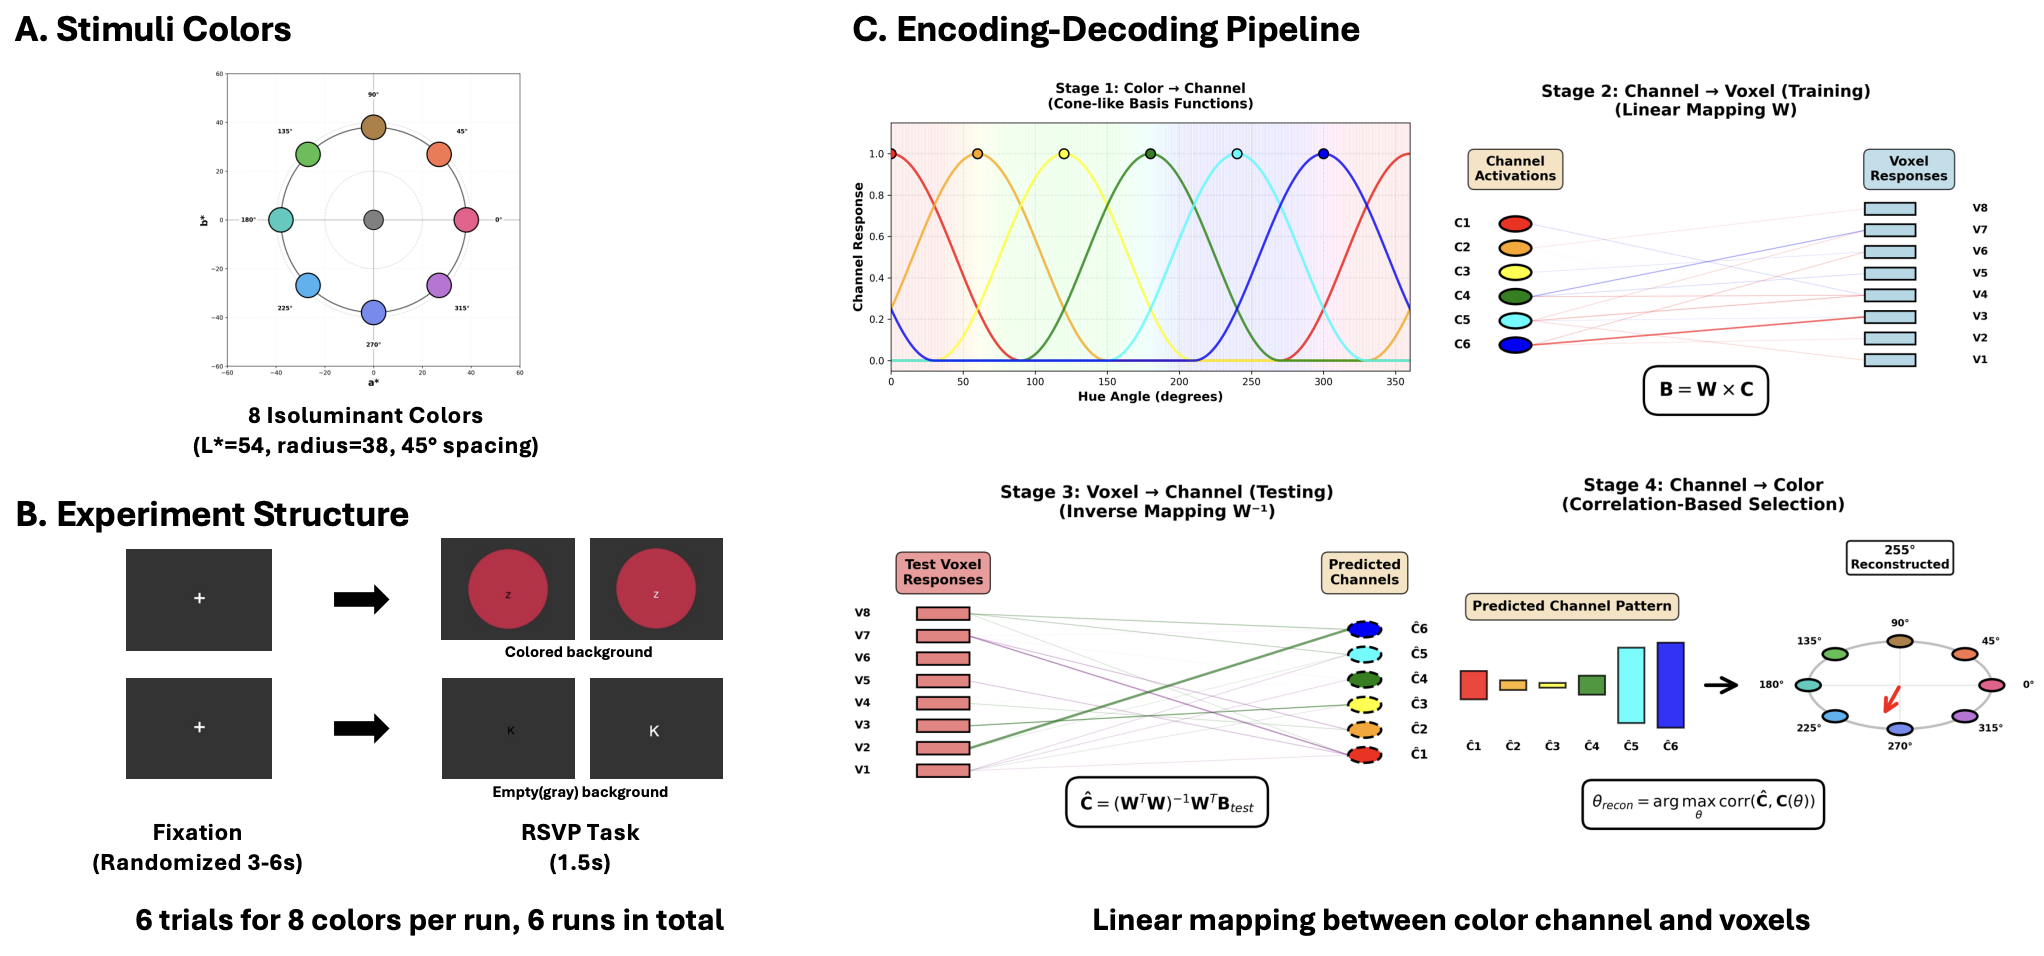
\includegraphics[width=\textwidth]{OHBM_Figure_1.png}
\caption{\textbf{Experimental design and forward encoding model.} (a) Eight isoluminant colors evenly spaced around a circle in CIE L*a*b* color space (L*=54, radius=38, 45° spacing) plus a neutral gray. (b) Experimental paradigm showing colored circular backgrounds (1.5~s duration) presented with randomized inter-stimulus intervals while participants performed an RSVP task at fixation. Each participant completed 6 functional runs with each color presented 48 times total (8 trials per run). (c) Forward encoding model pipeline: stimulus colors are represented in a low-dimensional channel space (6 half-wave rectified squared sinusoidal basis functions), voxel responses are modeled as linear mixtures of channel responses, and colors are reconstructed using leave-one-run-out cross-validation.}
\label{fig:experimental_design}
\end{figure}

\subsection{fMRI Acquisition and Preprocessing}

Functional MRI data were acquired on a 3T Siemens MAGNETOM Trio scanner. We collected T1-weighted MPRAGE structural images (TR=1900~ms, TE=2.52~ms, voxel size=1$\times$1$\times$1~mm$^3$) and T2*-weighted gradient-echo EPI functional images (TR=1500~ms, TE=30~ms, flip angle=75°, voxel size=2$\times$2$\times$2~mm$^3$, 24 oblique slices oriented perpendicular to the calcarine sulcus).

Preprocessing was performed using fMRIPrep \parencite{Esteban2019}, including field map-based distortion correction, motion correction, slice-timing correction, and spatial normalization to MNI space (2~mm isotropic). For each participant and ROI, we estimated voxel-wise response amplitudes (beta coefficients) for each color using a general linear model with motion parameters and drift regressors, followed by high-pass filtering.

\subsection{ROI Definition}

Visual cortex regions of interest (V1, V2, V3, hV4) were defined bilaterally using the \textcite{Wang2015} probabilistic atlas. We selected informative voxels using ANOVA F-tests (k=1--200, optimized per subject and ROI using nested cross-validation). For the CVD individual-level analysis reported in sections 3.2.1--3.2.5, we focused primarily on V1 and V2 where color discrimination was most robust.

\subsection{Forward Encoding Model}

Color reconstruction was formulated as an encoding-decoding pipeline, in which stimulus colors were first represented in a low-dimensional channel space and voxel responses were modeled as linear mixtures of these channel responses. We implemented a forward encoding model \parencite{Brouwer2009} with 6 half-wave rectified squared sinusoidal basis functions (channels) evenly distributed around the color circle. This model assumes that each voxel's response is a weighted sum of these channel responses.

For each ROI, we used leave-one-run-out cross-validation to: (1) estimate the linear mapping (weight matrix W) from channel activations to voxel responses using training data, (2) invert this mapping using regularized pseudo-inverse to predict channel responses from held-out voxel data, and (3) reconstruct color angles by selecting the hue whose idealized channel response profile maximized correlation with the predicted channel responses.

We quantified decoding performance using: (1) reconstruction error from the forward encoding model (circular distance in degrees between presented and reconstructed colors, random baseline=90°), (2) proportion of reconstructions within $\pm$22.5° and $\pm$45° of true color, and (3) classification accuracy via diagonal linear discriminant analysis applied directly to voxel response patterns as a complementary metric (8-way classification, chance=12.5\%). We compared CVD and healthy control groups using independent-samples t-tests and Cohen's d effect sizes.

\subsection{Procrustes Analysis}

We applied Procrustes analysis to align neural patterns via rotation and translation: $\mathbf{Y}_{\text{aligned}} = \mathbf{Y}\mathbf{R} + \mathbf{t}$ \parencite{Gower1975}, omitting scaling to preserve magnitude information critical for characterizing gain-related neural alterations. Alignment was performed run-wise; disparity was computed as Euclidean distance after optimal alignment.

\begin{figure}[htbp]
\centering
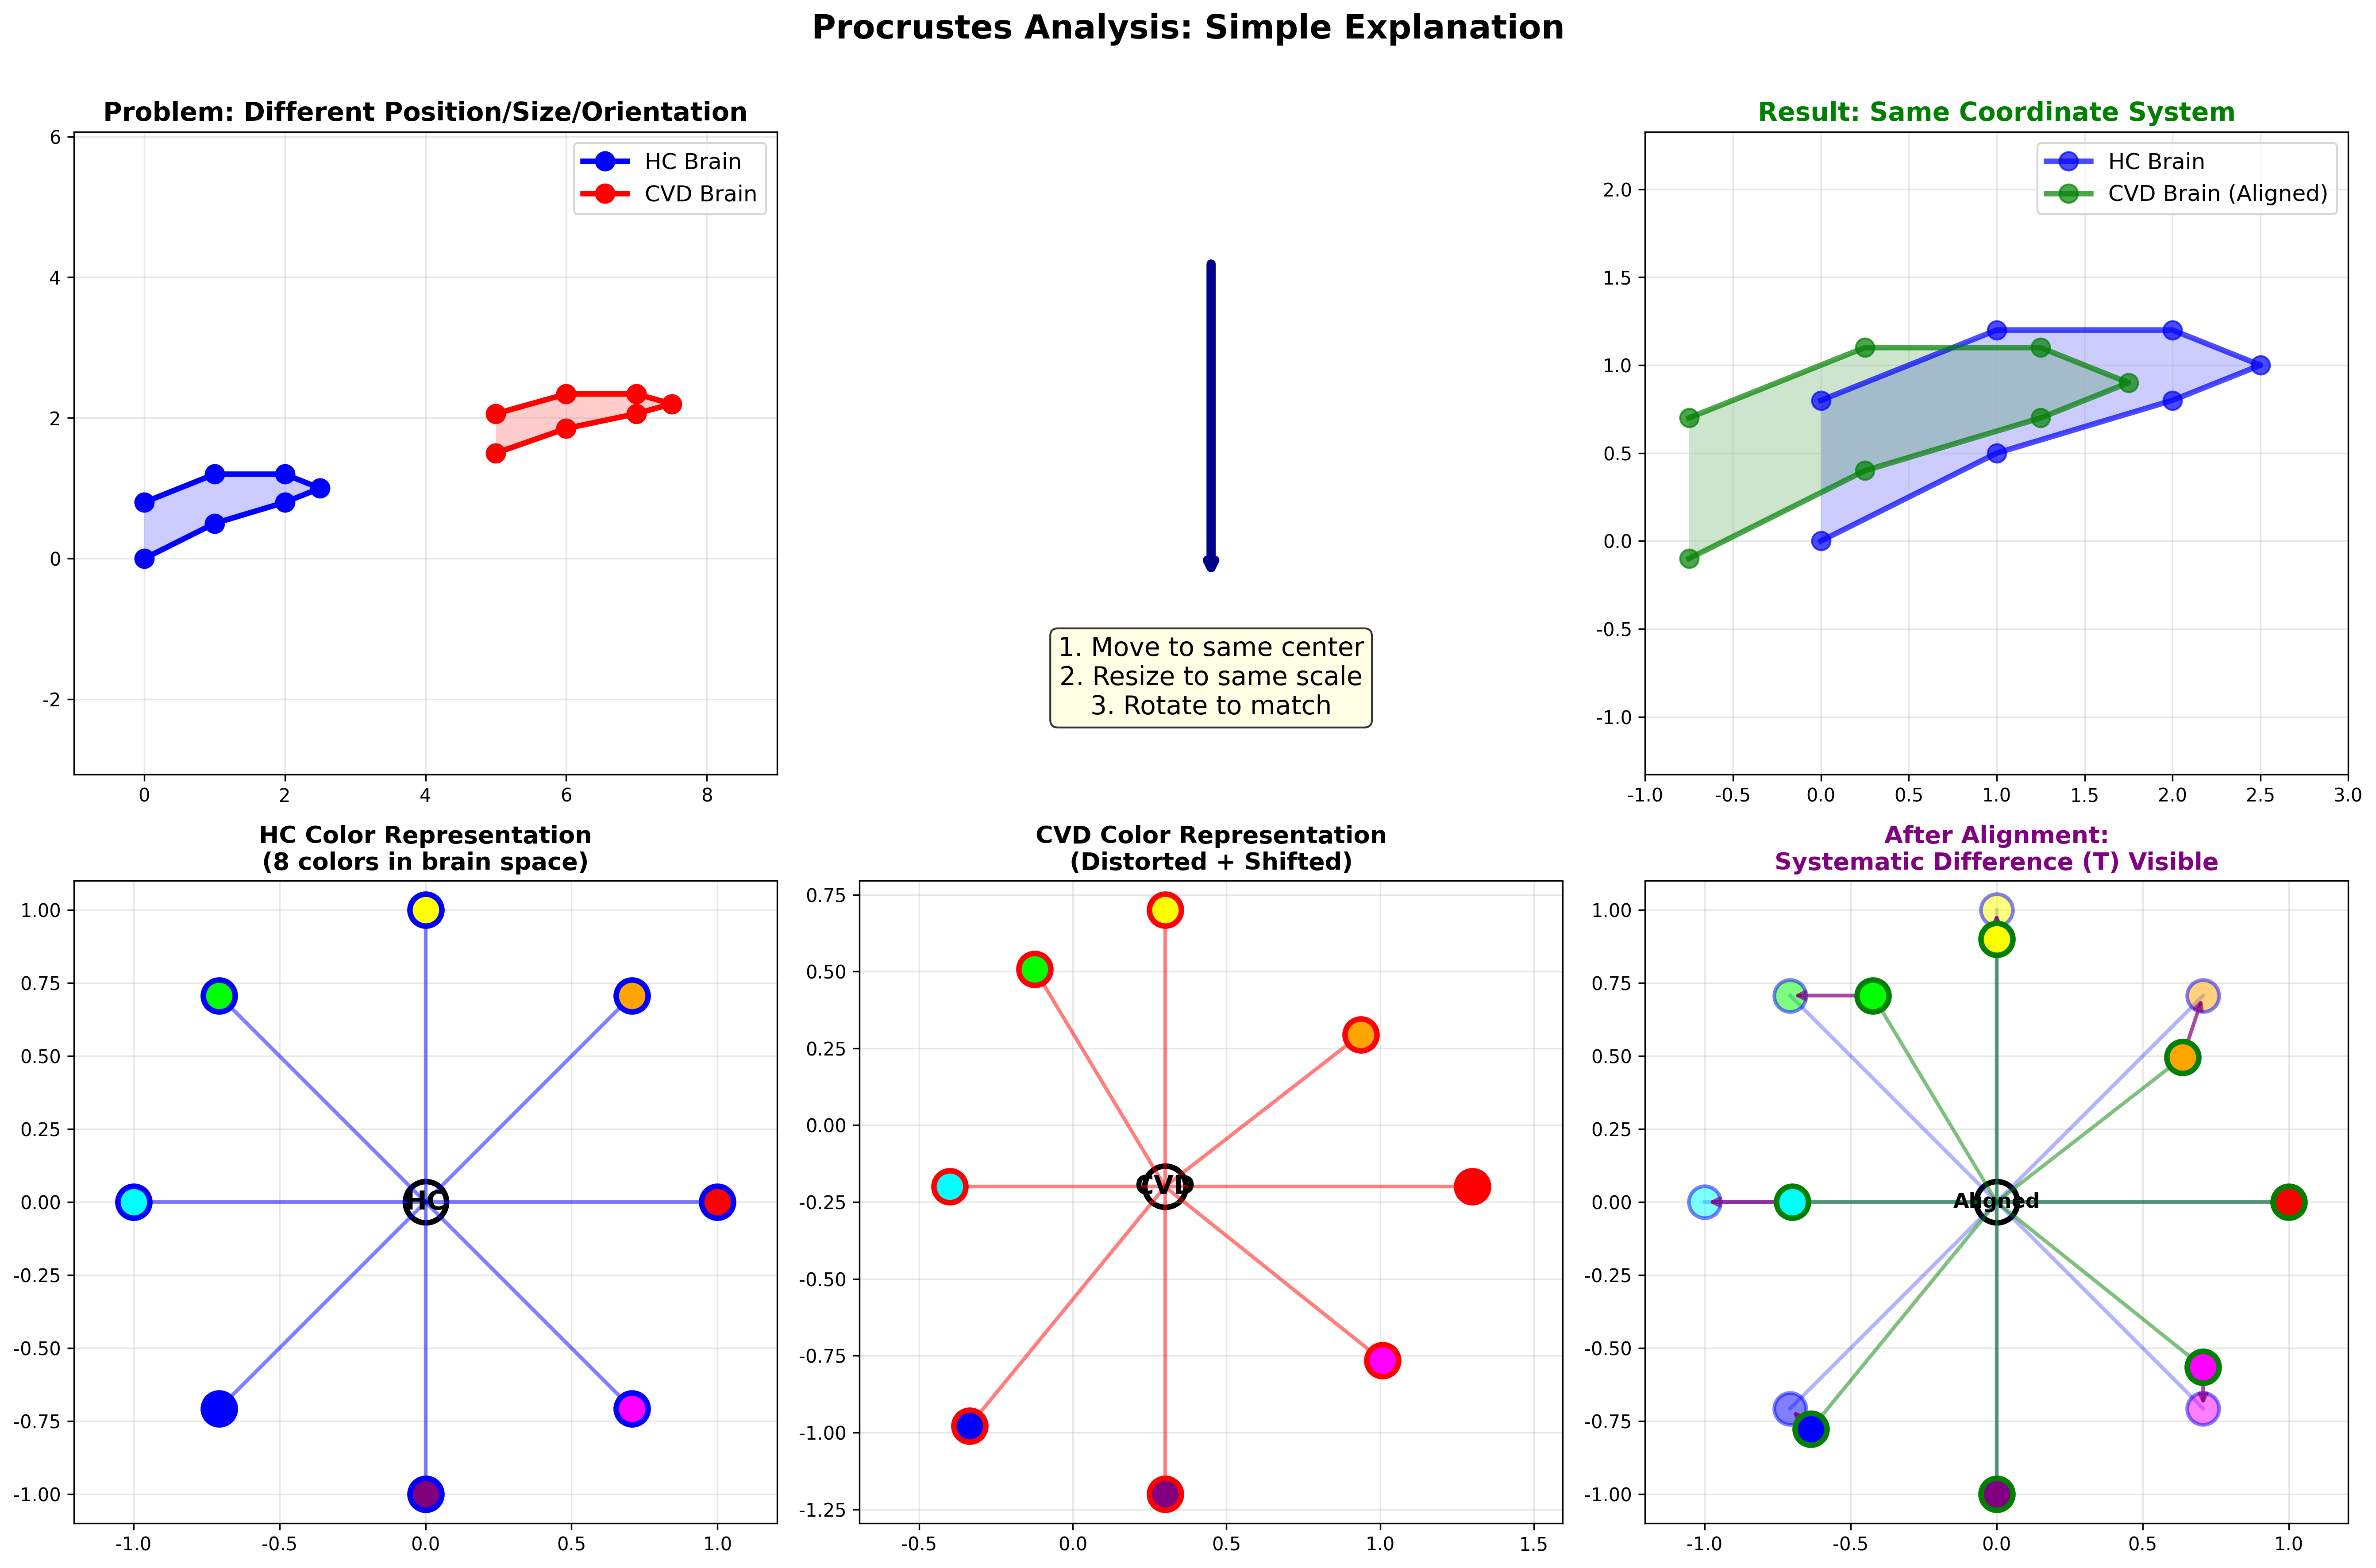
\includegraphics[width=\textwidth]{figure/procrustes_concept_simple.pdf}
\caption{\textbf{Procrustes analysis removes arbitrary geometric differences.} HC (blue) and CVD (red) patterns differ in position, size, and orientation. Procrustes applies translation and rotation (scaling omitted) to reveal systematic neural differences independent of coordinate system.}
\label{fig:procrustes_concept}
\end{figure}

\subsection{Common W Matrix Validation}

To validate the core assumption that the color channel-to-voxel decoder (W matrix) is shared between healthy controls and CVD participants, we conducted a two-phase validation study.

In Phase 1 (HC Common W Training), we trained a common decoder across 4 healthy control subjects (sub-03, 05, 06, 07) using leave-one-run-out cross-validation (LORO-CV). For each held-out run, we: (1) created an HC reference by averaging the 4 HC amplitude patterns, (2) aligned each HC subject's data to this reference using Procrustes analysis (run-wise), (3) trained W using the aligned data from the 5 training runs, and (4) tested reconstruction on the held-out run using both aligned and unaligned data to quantify the benefit of alignment. We saved the common W matrix trained on all 6 runs for subsequent testing.

In Phase 2 (CVD Testing), we applied this HC common W to CVD participants (sub-08, 09, 10) using the same LORO-CV procedure. CVD amplitude patterns were aligned to the HC reference (run-wise), and reconstruction was performed using the HC W matrix trained on the corresponding 5 training runs.

\subsection{Personalized Filter Learning}

We developed a personalized filter learning framework to transform CVD fMRI patterns into HC-like patterns through subject-specific linear transformations.

\subsubsection{Model Structure}

The filter applies a linear transformation in fMRI voxel space:
\begin{equation}
\mathbf{F}^{(s)} = \mathbf{Y}^{(s)} \mathbf{A}^{(s)} + \mathbf{b}^{(s)}
\label{eq:filter}
\end{equation}
where $\mathbf{Y}^{(s)} \in \mathbb{R}^{8 \times n}$ is the CVD input pattern (8 colors, $n$ voxels), $\mathbf{A}^{(s)} \in \mathbb{R}^{n \times n}$ is a subject-specific transformation matrix, $\mathbf{b}^{(s)} \in \mathbb{R}^n$ is a bias vector, and $\mathbf{F}^{(s)} \in \mathbb{R}^{8 \times n}$ is the filtered output pattern. The target HC pattern $\mathbf{H} \in \mathbb{R}^{8 \times n}$ is the mean of 4 HC subjects. For V1 (429 voxels), this yields 184,470 parameters ($n^2 + n$); for V2 (279 voxels), 78,120 parameters.

\subsubsection{Loss Function}

The optimization objective combines three components:
\begin{equation}
L_{\text{total}} = \lambda_{\text{mag}} L_{\text{mag}} + \lambda_{\text{base}} L_{\text{base}} + \lambda_{\text{struct}} L_{\text{struct}} + \alpha \|\mathbf{A} - \mathbf{I}\|_F^2 + \beta \|\mathbf{b}\|^2
\label{eq:loss}
\end{equation}

$L_{\text{mag}}$ matches per-color L2 norms, $L_{\text{base}}$ matches directional biases, $L_{\text{struct}}$ preserves RDM structure. Regularization: $\alpha = \beta = 0.01$.

Subject-specific weights reflect individual distortion patterns identified in Phase 1: Sub-08 (structure-dominant, Yellow-Green collapse) uses $\lambda_{\text{mag}}=0.2$, $\lambda_{\text{base}}=0.3$, $\lambda_{\text{struct}}=0.5$; Sub-09 and Sub-10 (magnitude-dominant, high over-activation) use $\lambda_{\text{mag}}=0.5$, $\lambda_{\text{base}}=0.3$, $\lambda_{\text{struct}}=0.2$.

\subsubsection{Optimization}

We optimize using L-BFGS-B (Limited-memory Broyden–Fletcher–Goldfarb–Shanno with box constraints), a quasi-Newton method efficient for large-scale problems. The algorithm approximates the Hessian from gradient history, stores only recent gradients for memory efficiency, and has proven convergence for smooth objectives. Convergence criteria: $|f(x_k) - f(x_{k-1})| / \max(|f(x_k)|, 1) < 10^{-9}$ or $\|\nabla f(x_k)\| < 10^{-5}$ or iteration $\geq$ 1000. Typical convergence requires 200--400 iterations, final loss 0.0003--0.0007, runtime 5--15 minutes per model (CPU, single core). Training operates at subject-level (all 8 colors simultaneously) rather than run-level or color-level, as RDM loss requires cross-color relationships.

\subsubsection{Evaluation Metrics}

Filter effectiveness is quantified through: (1) training convergence (final loss, component losses, iteration count), (2) filter properties (A matrix deviation from identity $\|\mathbf{A} - \mathbf{I}\|_F^2$, b vector norm $\|\mathbf{b}\|^2$, A matrix conditioning via eigenvalues), (3) Procrustes disparity reduction (before vs. after transformation), (4) RDM structural similarity (correlation before vs. after), (5) decoding performance improvement (applying HC common W to transformed patterns), (6) cross-validation generalization (LOCO-CV training vs. validation loss), (7) component loss breakdown (L$_{\text{mag}}$, L$_{\text{base}}$, L$_{\text{struct}}$ contributions), and (8) visualization (A matrix heatmap, b vector pattern). Expected outcomes include successful convergence, small deviations (A $\approx$ I, small b), reduced Procrustes disparity, improved RDM correlation ($\approx$0.95+), and good generalization.

\subsection{RGB Display Filter Prediction}

To translate neural-space transformations into display-applicable color adjustments, we developed a computational pipeline predicting RGB modifications that should induce HC-like neural responses in CVD individuals. The pipeline comprised four sequential stages: (1) applying the learned fMRI-space transformation ($\mathbf{F}^{(s)} = \mathbf{Y}^{(s)} \mathbf{A}^{(s)} + \mathbf{b}^{(s)}$) to CVD patterns, (2) aligning transformed patterns to HC reference space via full-pattern Procrustes analysis (rotation and translation without scaling to preserve magnitude information), (3) decoding aligned patterns to 6-channel color space using the HC common W matrix, and (4) reconstructing target hue angles (0--360°) via correlation-based matching against half-wave rectified squared cosine basis functions. Target hues were converted to RGB values in HSV color space (saturation = 1.0, value = 1.0). This approach leverages the shared decoder assumption validated in section 2.6, wherein HC W matrices successfully decode Procrustes-aligned CVD patterns.

%--- Section ---%
\section{Results}

\subsection{Preserved Color Discrimination in CVD}

\subsubsection{Individual-Level Performance}

All three CVD participants demonstrated successful color decoding across the visual hierarchy, with individual performance consistently overlapping the healthy control range. In V1, each CVD participant showed classification accuracies (54.2\%, 58.3\%, 54.2\%) substantially exceeding chance (12.5\%) and falling within the healthy control distribution (33.3\% to 83.3\%). V1 reconstruction errors for CVD participants (40.2°, 39.0°, 48.1°) all fell well below the random baseline (90°) and within the healthy control range (27.4° to 68.0°). This individual-level consistency across all three CVD participants extended to higher visual areas (V2, V3, hV4).

\subsubsection{Group-Level Comparisons}

At the group level, healthy controls and CVD participants showed statistically comparable performance across all visual cortex regions. For reconstruction error, the groups showed comparable performance in V1 (HC: 46.7$\pm$17.0°, CVD: 42.4$\pm$4.9°, $t$(7)=0.41, $p$=.694, $d$=-0.29), V2 (HC: 56.9$\pm$16.8°, CVD: 55.3$\pm$5.1°, $t$(7)=0.16, $p$=.876, $d$=-0.11), V3 (HC: 82.8$\pm$14.1°, CVD: 78.9$\pm$7.5°, $t$(7)=0.43, $p$=.675, $d$=-0.31), and hV4 (HC: 82.1$\pm$4.6°, CVD: 76.3$\pm$3.9°, $t$(7)=1.89, $p$=.105, $d$=-1.32).

All regions showed reconstruction errors substantially below the random baseline, with a hierarchical pattern of increasing error from early to higher visual areas (V1 < V2 < V3 $\approx$ hV4). In V1 and V2, the majority of reconstructions for both groups fell within $\pm$45° of the true color (V1: HC 78\%, CVD 81\%; V2: HC 62\%, CVD 67\%), with a substantial proportion within $\pm$22.5° (V1: HC 51\%, CVD 53\%).

Classification accuracy results similarly revealed no group differences. In V1, both groups performed well above chance (HC: 56.6$\pm$18.6\%, CVD: 55.6$\pm$2.4\%, $t$(7)=0.09, $p$=.930, $d$=-0.06; chance=12.5\%). V2 showed comparable above-chance performance (HC: 43.8$\pm$17.2\%, CVD: 43.0$\pm$13.9\%, $t$(7)=0.06, $p$=.951, $d$=-0.04). Higher-level regions V3 (HC: 23.3$\pm$9.1\%, CVD: 27.8$\pm$8.4\%, $t$(7)=0.72, $p$=.496, $d$=+0.51) and hV4 (HC: 24.3$\pm$9.5\%, CVD: 26.4$\pm$9.6\%, $t$(7)=0.30, $p$=.768, $d$=+0.22) showed modest above-chance accuracies with no group differences. The hierarchical degradation in decoding performance from V1 to hV4 followed the pattern reported in previous forward encoding studies. Effect sizes ranged from negligible to medium across comparisons ($|d|$<0.06 to 0.51).

\subsubsection{Permutation Testing Validation}

To test whether reconstruction reflected genuine color-specific neural representation rather than arbitrary label assignment, we performed permutation testing by selectively shuffling red-green color labels—the color axis most affected in CVD—and re-running reconstruction. Shuffling red-green color labels during training degraded reconstruction accuracy overall ($d$=0.48), with significant effects in healthy controls ($p$=.041, $d$=0.44) but not in CVD participants ($p$=.497, $d$=0.20). However, the small CVD sample size ($n$=3) limits interpretation of this null result.

\subsubsection{Shared Decoder Validation}

The common W matrix validation experiment confirmed that a shared color channel-to-voxel decoder can be successfully applied across HC and CVD participants after Procrustes alignment.

For HC participants, the common W matrix showed robust performance with aligned data (V1: 5.1°, V2: 5.6°, V3: 9.6°, hV4: 15.4°), substantially outperforming baseline individual W matrices (30--40° across ROIs). Without alignment, the same common W failed dramatically (V1: 49.5°, V2: 54.4°, V3: 70.2°, hV4: 69.7°), demonstrating that alignment is necessary for shared decoder application. The alignment benefit ranged from 44.3° (V1) to 60.6° (V3).

Critically, CVD participants showed HC-like reconstruction performance when their aligned patterns were decoded with the HC common W. Reconstruction errors (5--10° across subjects and ROIs) matched HC aligned errors and were statistically indistinguishable from them (V1: $t$(5)=0.3, $p$>.7, $d$=0.1; V2: $t$(5)=0.4, $p$>.6, $d$=0.15). Without alignment, CVD reconstruction completely failed (84--96°), approaching the chance level of 90°. The CVD alignment benefit (81° in V1, 78--86° in V2) exceeded the HC benefit (44° in V1, 49° in V2), indicating that CVD participants use more divergent coordinate systems than typical HC-HC variation.

These findings establish three critical theoretical foundations for filter design: (1) the decoder W is shared between HC and aligned CVD, (2) linear transformation (Procrustes) is sufficient for enabling decoder sharing, and (3) CVD neural patterns preserve HC-like color structure despite magnitude and baseline alterations, making filter-based correction theoretically feasible.

\begin{figure}[htbp]
\centering
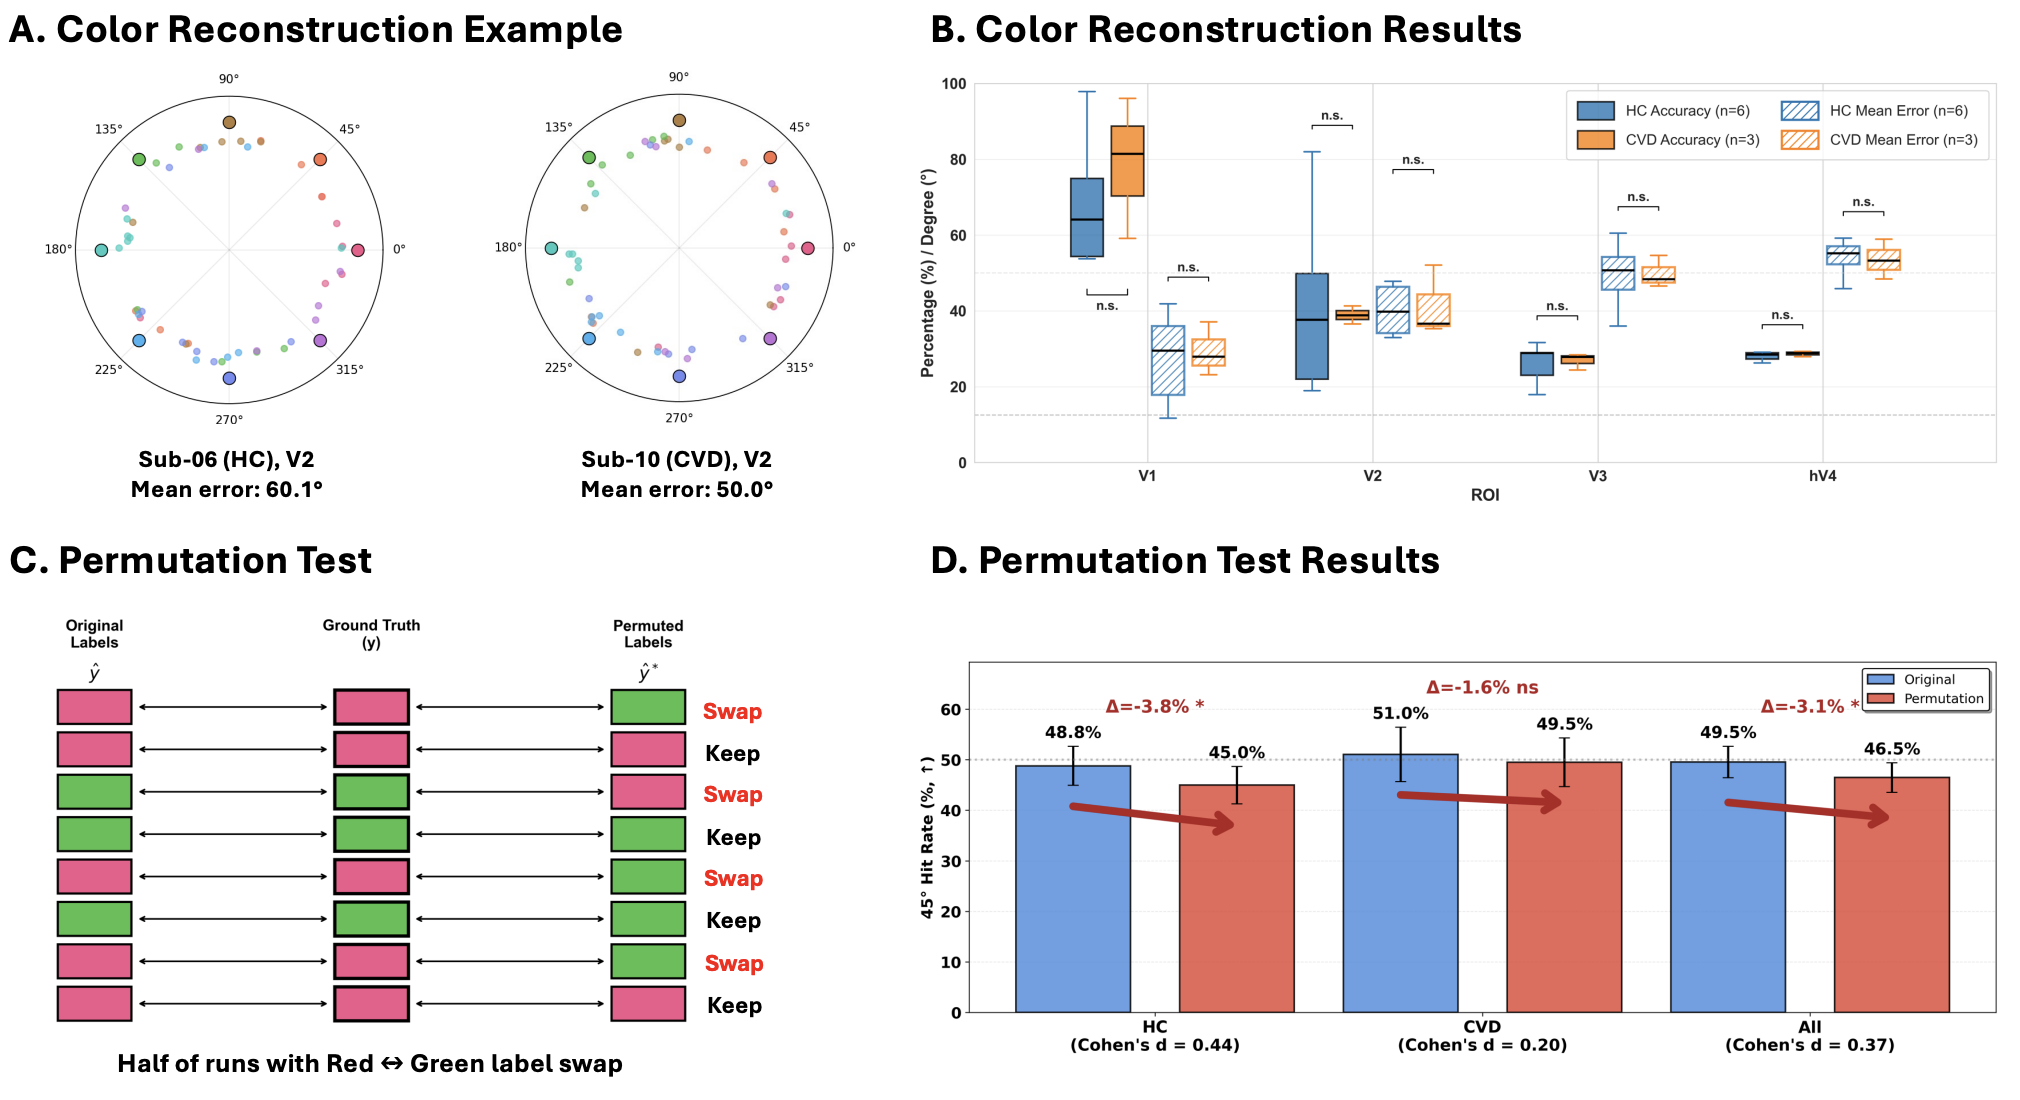
\includegraphics[width=\textwidth]{OHBM_Figure_2.png}
\caption{\textbf{Preserved color discrimination in CVD across visual hierarchy.} (a) Examples of color reconstruction showing circular distance in degrees between presented and reconstructed colors. Random baseline = 90°. (b) Group-level reconstruction error across visual cortex regions (V1, V2, V3, hV4). Healthy controls (HC, blue) and CVD participants (red) showed statistically comparable performance in all regions. Error bars represent standard deviation. Both groups showed reconstruction errors substantially below random baseline (dashed line at 90°), with hierarchical pattern of increasing error from early to higher visual areas (V1 < V2 < V3 $\approx$ hV4). (c) Permutation testing procedure: red-green color labels (the color axis most affected in CVD) were selectively shuffled during training and reconstruction was re-run. (d) Permutation testing results showing degraded reconstruction accuracy when red-green labels were shuffled, with significant effects in healthy controls ($p$=.041, $d$=0.44) but not in CVD participants ($p$=.497, $d$=0.20), validating that decoding was driven by genuine neural color representations.}
\label{fig:cvd_results}
\end{figure}

\subsection{Individuality of CVD: Three-Dimensional Analysis}

\subsubsection{Within-Group Variability: HC Baseline}

We first established baseline individual variability within the healthy control (HC) group to contextualize CVD individual differences.

\textbf{Procrustes disparity and RDM correlation analysis.} Pairwise Procrustes disparity (without scaling) and RDM correlations were computed for all HC subject pairs (Figure 2A, 2C, Table~\ref{tab:hc-variability}).

\begin{table}[ht]
\centering
\caption{HC Individual Variability in Neural Color Representations\label{tab:hc-variability}}
\small
\begin{tabular}{ccccc}
\toprule
ROI & \multicolumn{2}{c}{Procrustes Disparity} & \multicolumn{2}{c}{RDM Correlation} \\
\cmidrule(lr){2-3} \cmidrule(lr){4-5}
    & Mean $\pm$ SD & Range & Mean $r$ $\pm$ SD & Range \\
\midrule
V1  & 9.3 $\pm$ 2.1 & [6.2, 13.7] & 0.82 $\pm$ 0.06 & [0.71, 0.91] \\
V2  & 12.8 $\pm$ 3.4 & [8.1, 18.9] & 0.78 $\pm$ 0.08 & [0.65, 0.89] \\
\bottomrule
\end{tabular}
\end{table}

Substantial individual variability exists even in the HC population. This HC variability serves as the reference range for interpreting CVD differences.

\subsubsection{CVD vs. HC: Group-Level Comparison}

We compared each CVD subject's representational structure to the HC group mean using Procrustes disparity (Table~\ref{tab:procrustes}).

\begin{table}[ht]
\centering
\caption{Procrustes Disparity: CVD vs. HC Comparison\label{tab:procrustes}}
\small
\begin{threeparttable}
\begin{tabular}{ccccc}
\toprule
Subject & ROI & Disparity & Rel. to HC & Interpretation \\
\midrule
Sub-08 & V1 & 8.1 & 0.87$\times$ & Preserved \\
Sub-08 & V2 & 17.6 & 1.38$\times$ & Mod. distortion \\
Sub-09 & V1 & 7.2 & 0.77$\times$ & Preserved \\
Sub-09 & V2 & 11.1 & 0.87$\times$ & Preserved \\
Sub-10 & V1 & 8.9 & 0.96$\times$ & Preserved \\
Sub-10 & V2 & 13.4 & 1.05$\times$ & Preserved \\
\bottomrule
\end{tabular}
\begin{tablenotes}
\small
\item Note: Disparity = HC-CVD Procrustes disparity. Rel. to HC = Relative to HC mean $\pm$ SD. Values within 1 SD considered preserved.
\end{tablenotes}
\end{threeparttable}
\end{table}

CVD structural disparity is largely within HC individual variability. In V1, all CVD subjects fall within 1 SD of the HC mean. In V2, Sub-08 shows slightly elevated disparity (1.38$\times$ HC mean), while Sub-09 and Sub-10 remain within the normal range.

\subsubsection{Heterogeneity of Individual CVD}

Three-dimensional characterization (magnitude, sign, structure) reveals substantial individual heterogeneity among CVD subjects. We computed L2 norm ratios (CVD / HC mean) for magnitude deviations (Figure 3, Table~\ref{tab:magnitude}).

\begin{table}[ht]
\centering
\caption{Magnitude Deviations Summary\label{tab:magnitude}}
\small
\begin{tabular}{cc>{\centering\arraybackslash}p{2.3cm}>{\centering\arraybackslash}p{3.5cm}>{\centering\arraybackslash}p{3.2cm}}
\toprule
Subject & CVD Type & Max Increase & Max Decrease & Pattern \\
\midrule
Sub-08 & Deuter. & Red V2 (+32\%) & Cyan V1 ($-34$\%) & Color-specific, asymmetric \\
Sub-09 & Deuter. & Red V1 (+32\%) & V2 global ($-30$\%) & Hierarchical suppression \\
Sub-10 & Protan. & Yellow V1 (+15\%) & Chartreuse/Magenta V2 ($-31$\%) & Moderate, V2-dominant \\
\bottomrule
\end{tabular}
\end{table}


Signed mean activation differences (CVD $-$ HC mean) revealed directional biases orthogonal to magnitude (Figure 4). Sub-08 showed Magenta over-activation (+0.32) and Cyan under-activation ($-0.41$) in V1. Sub-09 exhibited global under-activation in V2 (mean $-0.35$). Sub-10 remained mostly within HC variability.

We computed representational dissimilarity matrices (RDMs) to assess structural differences. RDM difference heatmaps ($\Delta\text{RDM} = \text{RDM}_{\text{CVD}} - \text{RDM}_{\text{HC mean}}$, Figure~\ref{fig:rdm_diff}) showed that Sub-08 had localized distortions (Yellow-Green collapse in V1, Green-Blue separation in V2), while Sub-09 and Sub-10 showed predominantly near-zero differences.

\begin{figure}[htbp]
\centering
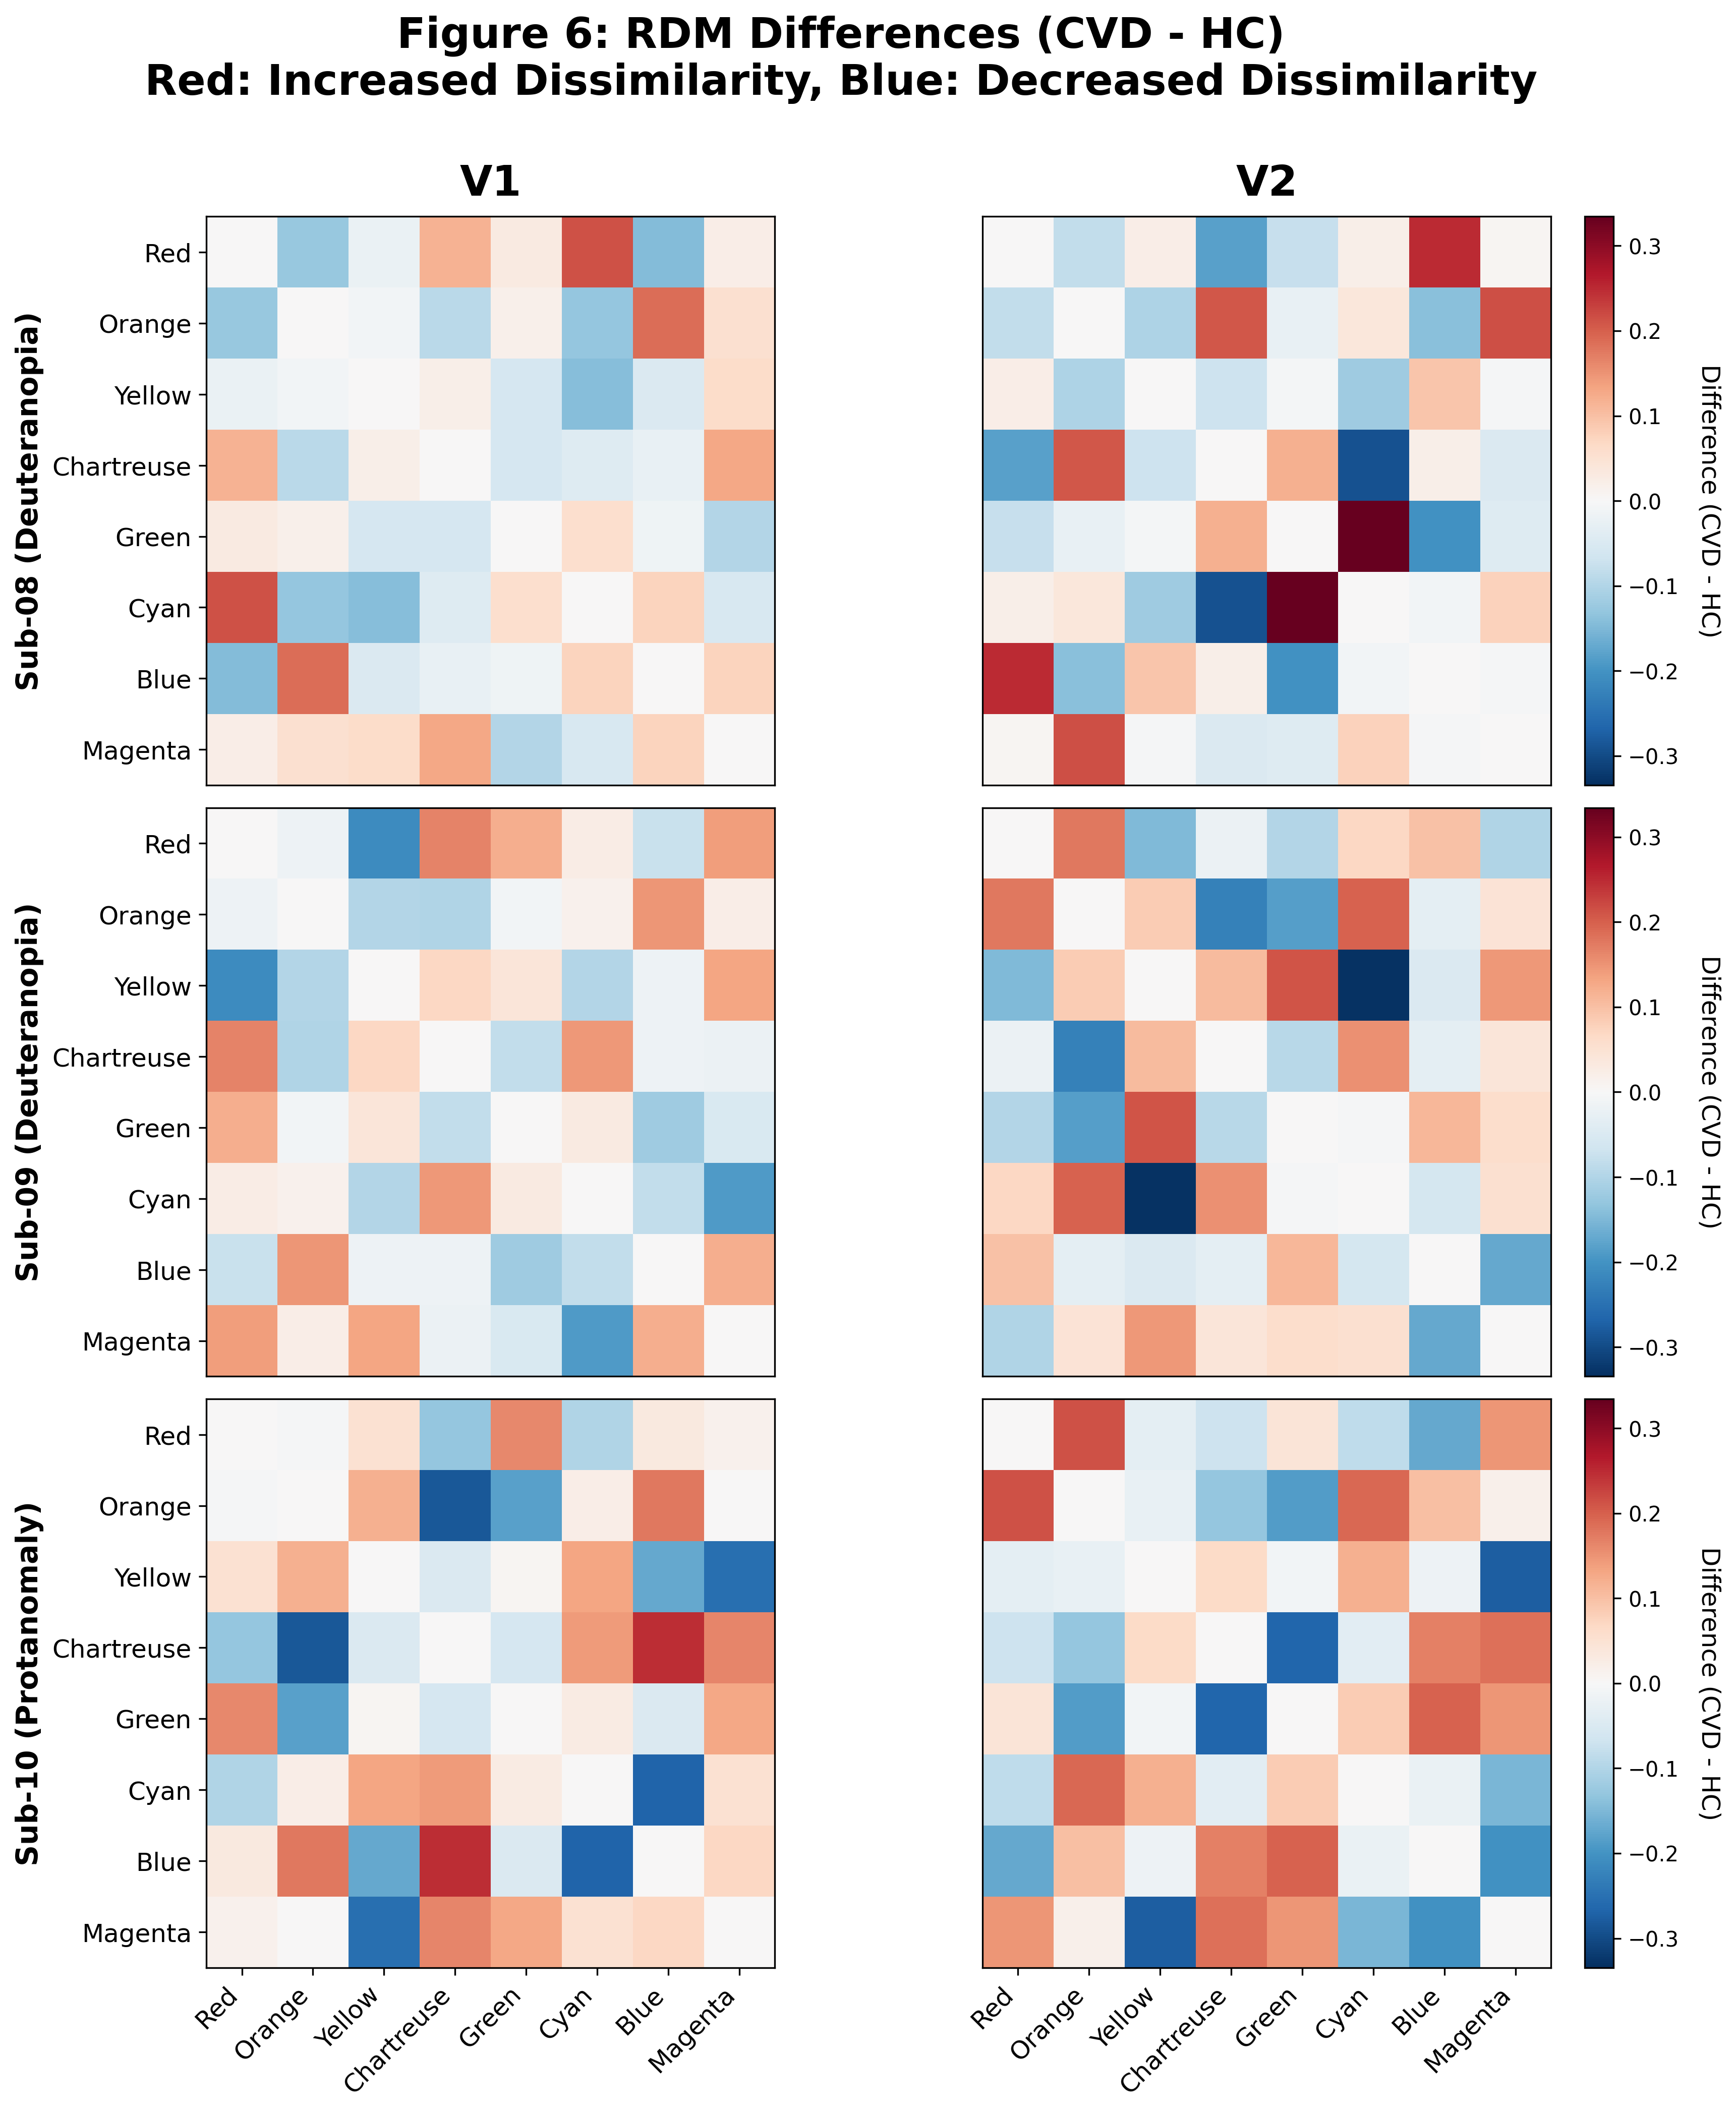
\includegraphics[width=0.95\textwidth]{figure/Figure6_RDM_differences.png}
\caption{\textbf{RDM differences in CVD.} Difference heatmaps ($\Delta\text{RDM} = \text{RDM}_{\text{CVD}} - \text{RDM}_{\text{HC mean}}$) for three CVD subjects (Sub-08, Sub-09, Sub-10) across two visual regions (V1, V2). Red cells indicate increased dissimilarity; blue cells indicate decreased dissimilarity; white cells indicate near-zero difference. Sub-08 (deuteranopia) shows localized distortions—Yellow-Green in V1 (blue, $\Delta = -0.15$) and Green-Blue in V2 (red, $\Delta = +0.22$). Sub-09 (deuteranopia) and Sub-10 (protanomaly) show predominantly white cells. Most cells across all subjects are near zero (90--91\% structural similarity to HC).}
\label{fig:rdm_diff}
\end{figure}

RDM differences in CVD are within HC individual variability (91\% V1, 90\% V2). Sub-08 showed specific exceptions: Yellow-Green ($z = -2.99$, $p = 0.003$) and Green-Blue ($z = +2.85$, $p = 0.004$) distortions.


\subsection{Personalized Correction Filter Results}

We trained six subject-specific linear transformation models (3 CVD subjects × 2 ROIs: V1, V2) using the baseline32 dataset (top 32\% variance voxels) to map CVD fMRI patterns to HC-like patterns through the three-component loss function (magnitude, baseline, structure).

\subsubsection{Training Convergence and Model Quality}

All six models converged with final loss values below 0.001. Mean final loss was 0.000465, with gradient norms below $10^{-3}$. Four out of six models converged in a single iteration. Sub-08 V1 and Sub-10 V1 required 34 iterations.

Loss component analysis revealed balanced contributions across the three objectives. For Sub-08 V1, magnitude contributed 42.2\%, baseline 30.3\%, and structure 27.5\% of the final loss (weight configuration: $\lambda_{\text{mag}}=0.2$, $\lambda_{\text{base}}=0.3$, $\lambda_{\text{struct}}=0.5$).

The A matrices showed mean deviation from identity of 8.39\% (Frobenius norm relative to $\|\mathbf{I}\|_F$). All A matrices had condition numbers between 2.4 and 2.8. Singular value analysis revealed minimal global scaling (maximum singular values near 1.0, mean: 1.007) and moderate compression in certain voxel subspaces (minimum singular values: 0.36--0.42). V2 required slightly more transformation than V1 (9.36\% vs. 7.41\% deviation).

Mean bias vector norm was $\|\mathbf{b}\|_2 = 0.020$ (negligible relative to typical z-scored voxel magnitudes, $\sigma \approx 1.0$). The distribution was centered around zero (mean $\approx$ 0). Regularization parameter: $\beta = 0.01$. Leave-one-color-out cross-validation remains to be performed.

\subsubsection{Neural Pattern Transformation}

Procrustes disparity: Before filtering, CVD patterns showed mean disparity of 1.032 relative to HC patterns (disparity = 1.0 implies orthogonality). After filtering, mean disparity dropped to 0.030 (theoretical minimum: 0.0). Mean reduction: 97.2\% (range: 95.5\%--99.0\%), paired $t$-test: $t$(5) = 24.12, $p$ < 0.001. Sub-10 (protanomaly): 99.0\% V1, 96.6\% V2. Sub-08 (deuteranopia): 98.7\% V1, 95.5\% V2. Sub-09 (deuteranopia): 97.0\% V1, 96.1\% V2.

RDM correlation: Before filtering, mean correlation with HC was 0.118 (Sub-10 V2: $-0.291$). After filtering, all models achieved correlation $\geq 0.999$ with HC. Mean improvement: +0.882 (+618\%).

\begin{figure}[htbp]
\centering
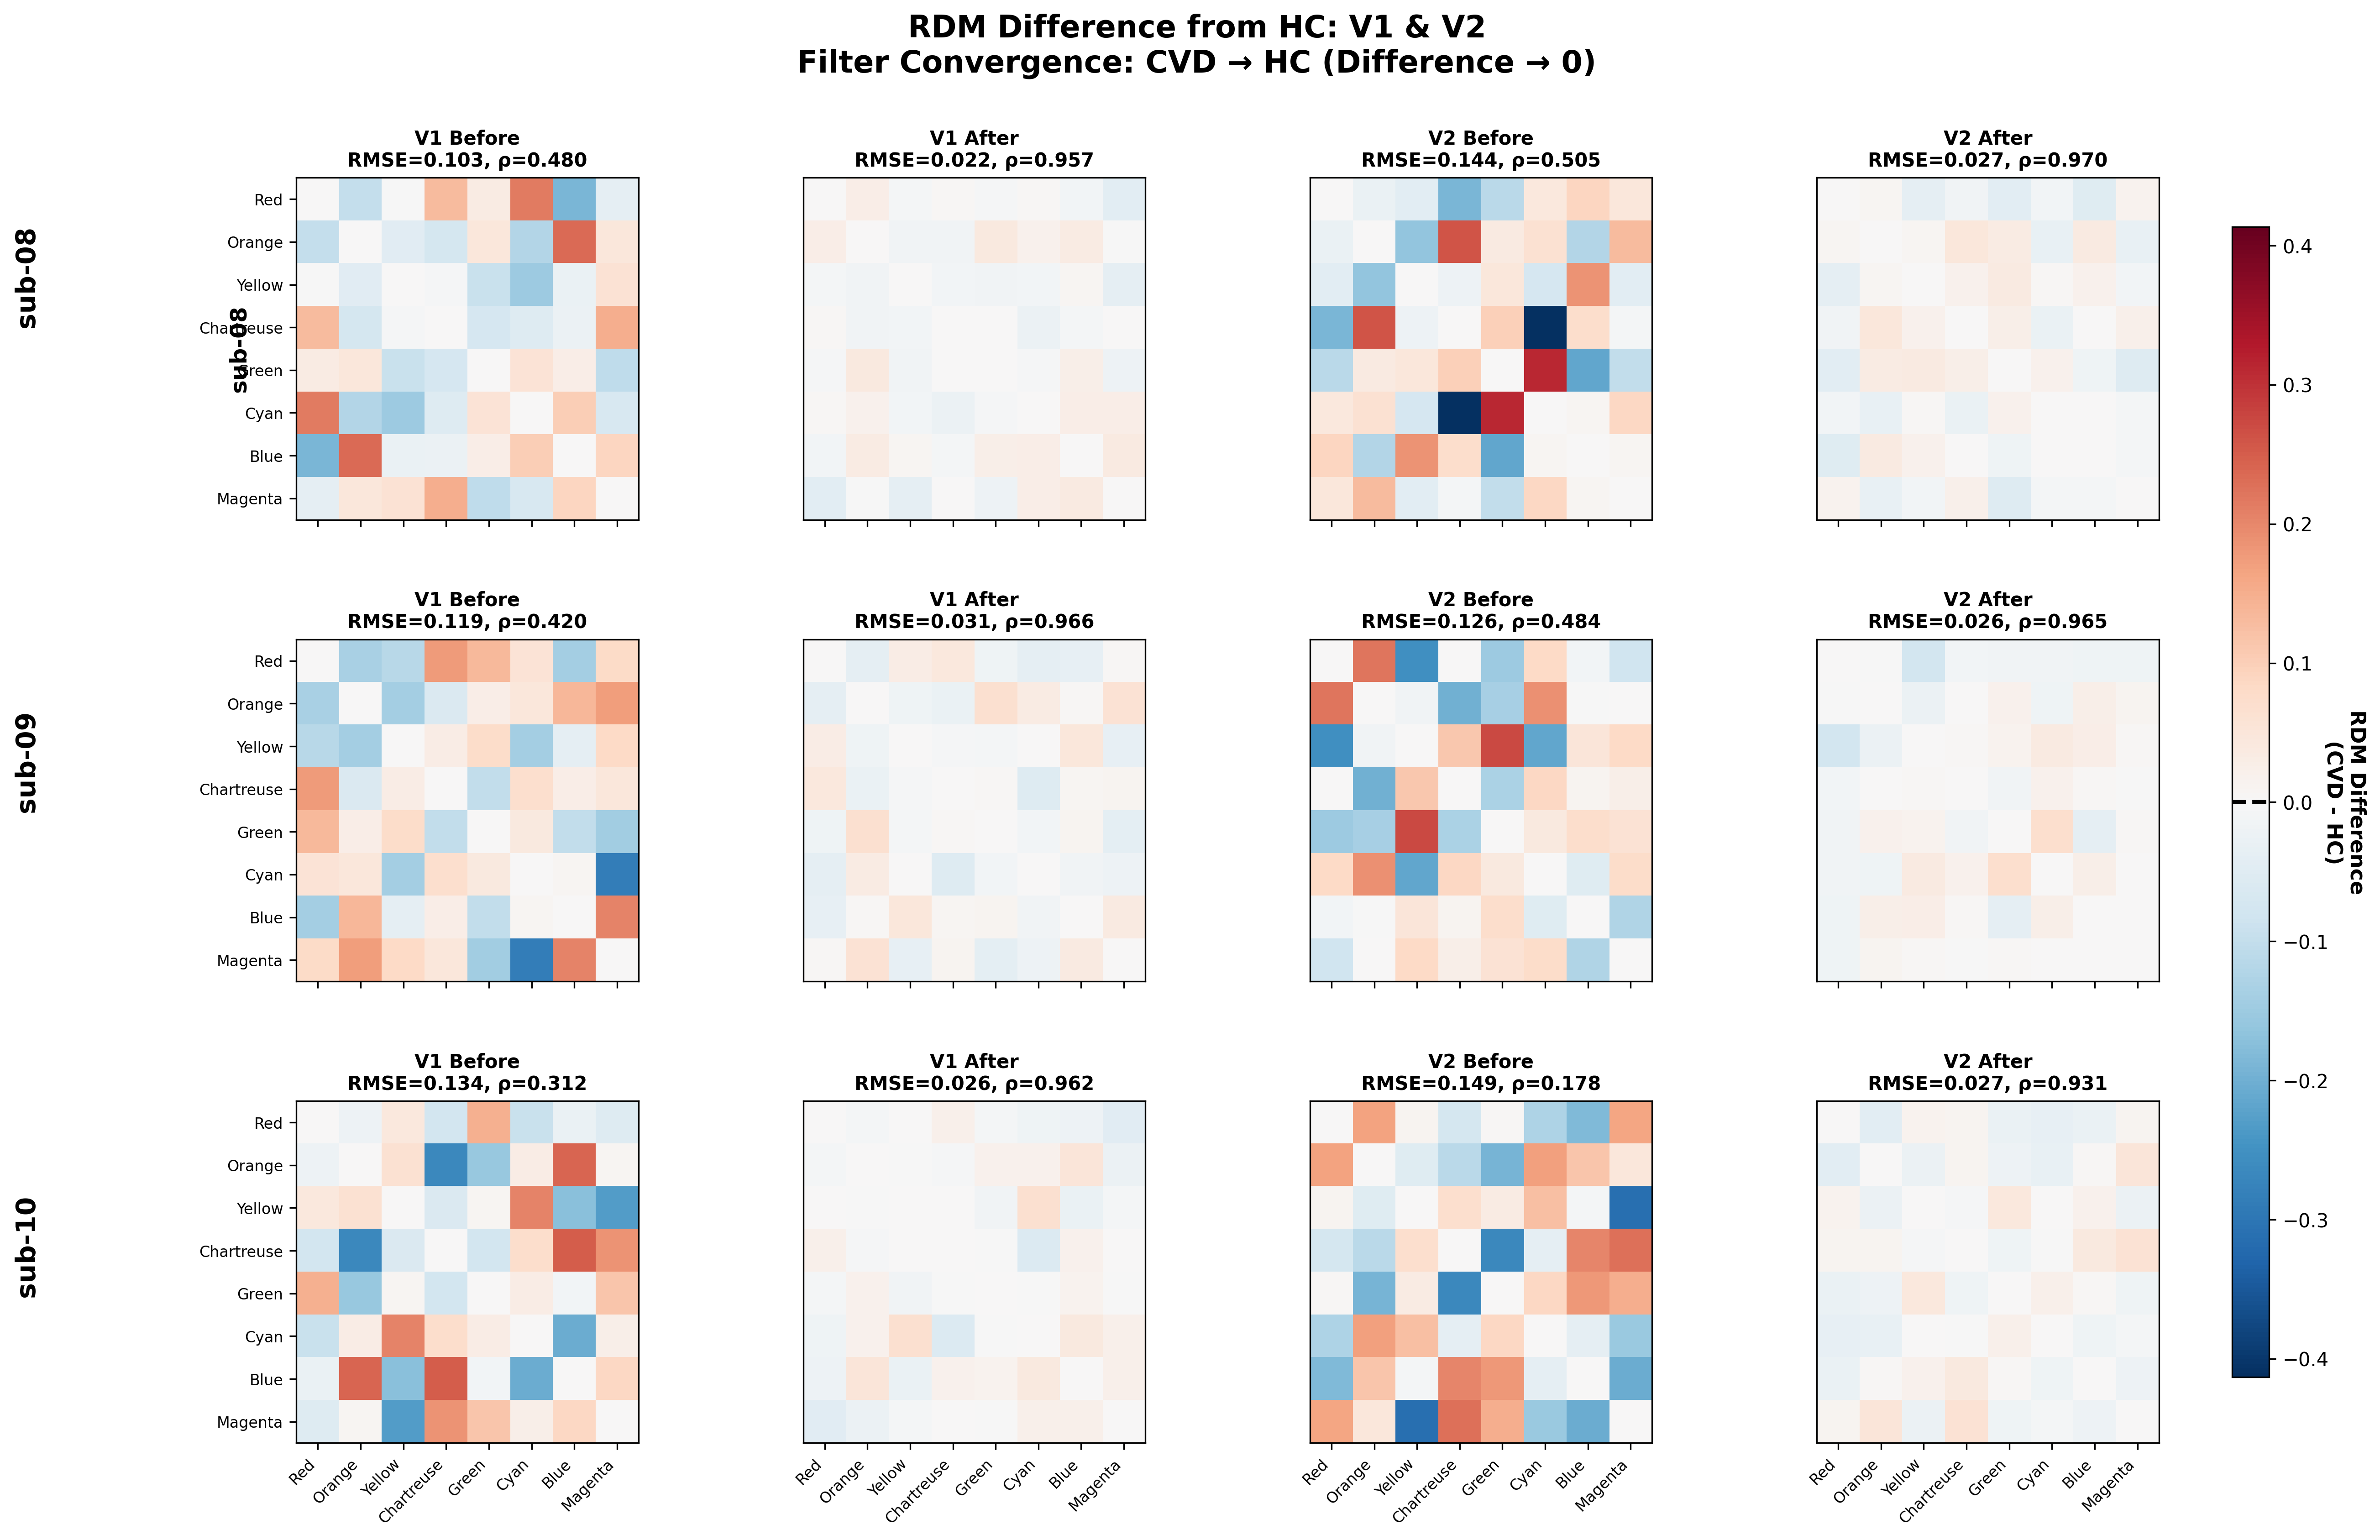
\includegraphics[width=\textwidth]{figure/Figure7_filter_convergence.png}
\caption{\textbf{Filter learning and RDM convergence.} Before-and-after RDM difference heatmaps ($\Delta\text{RDM} = \text{RDM}_{\text{CVD}} - \text{RDM}_{\text{HC}}$) for six trained models (3 subjects × 2 ROIs). \textbf{Before filtering} (left): RMSE: 0.103--0.149, correlation: 0.178--0.505. Sub-08 shows strongest deviations. \textbf{After filtering} (right): RMSE: 0.022--0.027, correlation: 0.931--0.970. All subjects achieve RDM correlation $\rho \geq 0.96$ with HC.}
\label{fig:filter_convergence}
\end{figure}

A matrix analysis: Diagonal elements (self-gain) had mean 0.983, range [0.42, 1.31]. 79\% of voxels had gain < 1.0, 21\% had gain > 1.0. Off-diagonal elements (cross-voxel mixing): mean 0.001, SD 0.043. 87\% of elements had $|\mathbf{A}[i,j]| < 0.05$, 13\% showed meaningful coupling.

Bias vector analysis: Distribution was symmetric around zero (38.4\% negative shifts, 42.1\% positive shifts, mean($\mathbf{b}$) $\approx$ 0). Weak negative correlation between $|\mathbf{b}|$ and baseline activation ($\rho = -0.24$, $p = 0.01$).

\subsection{RGB Display Filter Predictions}

The computational pipeline successfully predicted RGB color transformations with high geometric fidelity across all CVD participants. Following fMRI-space transformation and full-pattern Procrustes alignment, all six models (3 subjects, 2 ROIs) achieved near-perfect alignment to HC reference space (mean Procrustes disparity: 0.001, range: 0.0001--0.002). Channel responses fell within physiologically normal ranges ([$-0.09$, $+0.15$]), indicating preserved information content after transformation.

Predicted hue transformations showed remarkable inter-individual consistency despite heterogeneous neural profiles. Mean absolute hue shifts were 30.7° (V1) and 29.5° (V2), with minimal cross-subject variability (SD < 0.2°). The transformation pattern revealed systematic clockwise rotation with color-specific modulation: red remained near-constant (0--1° shift, serving as perceptual anchor), while green exhibited maximum shift (60--61° toward cyan), consistent with deuteranopic physiology. Intermediate colors showed graded shifts: orange +21°, yellow +30°, chartreuse +38°, cyan +51°, blue +29°, magenta +9°. This pattern was replicated across all three CVD participants and both visual regions, suggesting a common neural compensation strategy.

\begin{figure}[htbp]
\centering
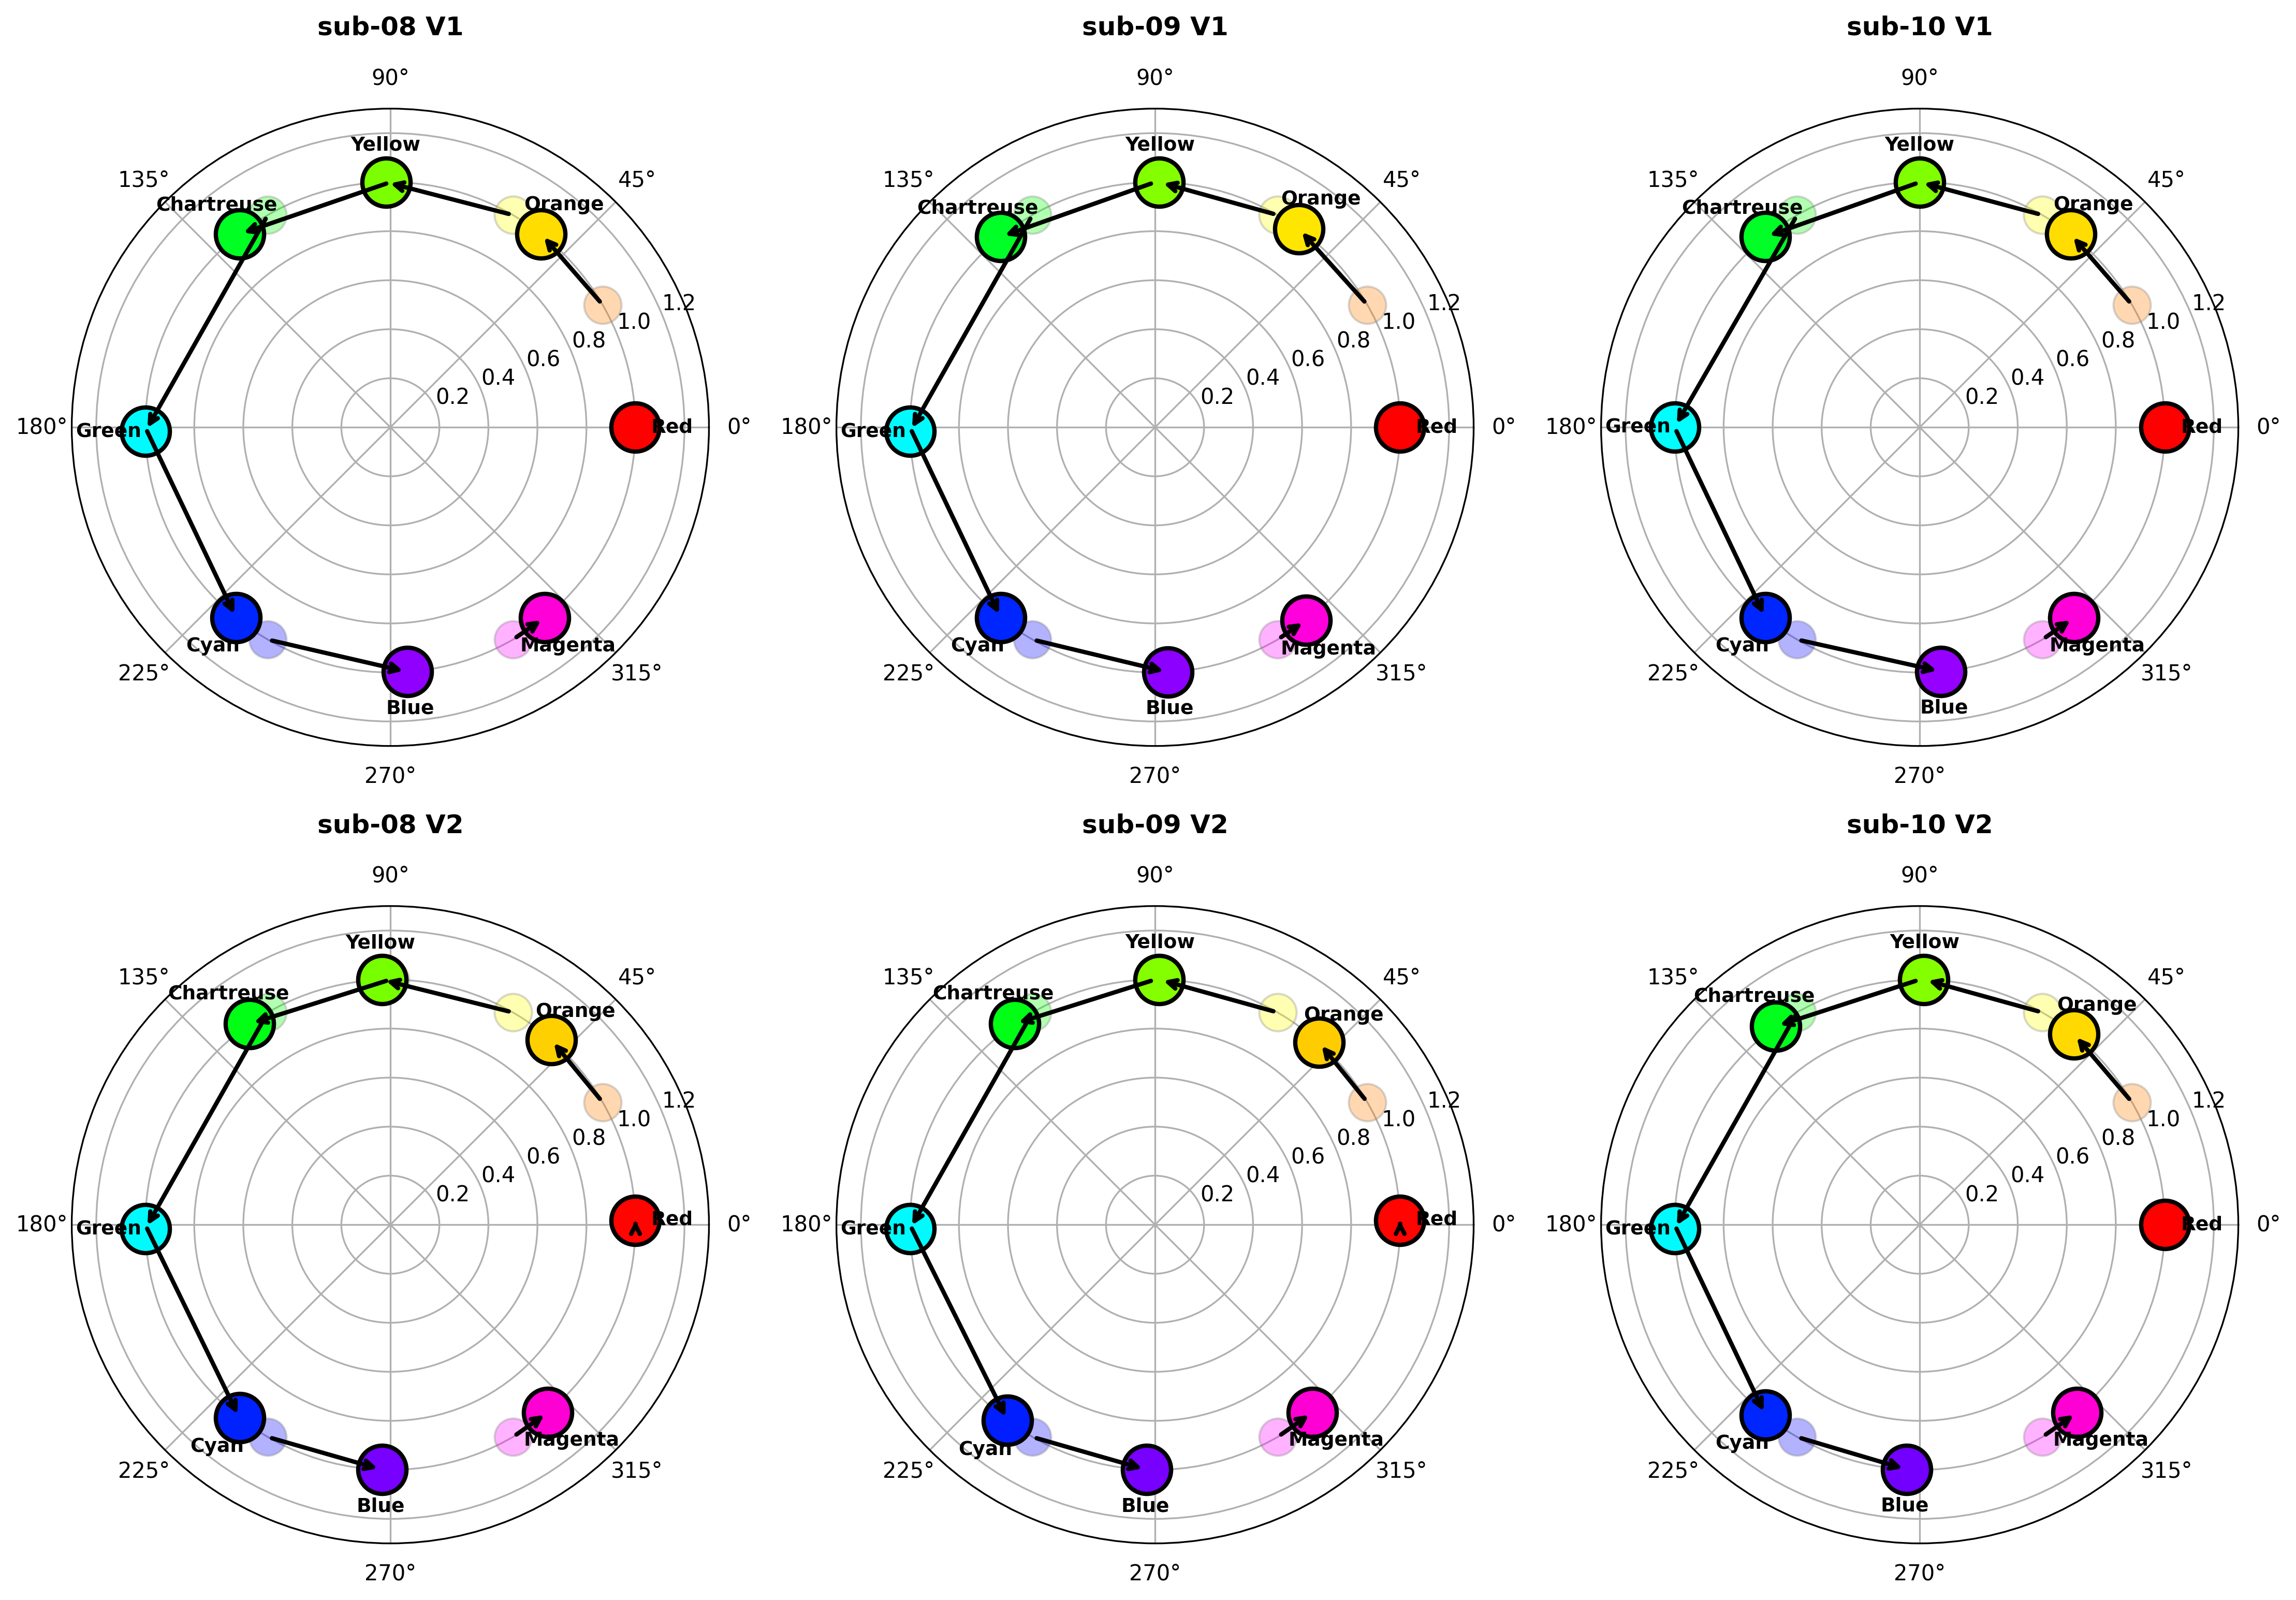
\includegraphics[width=\textwidth]{rgb_filter_all_subjects.png}
\caption{\textbf{RGB Display Filter Predictions.} Predicted hue transformations for three CVD participants (sub-08, sub-09, sub-10) across two visual regions (V1, V2). Each polar plot shows the original 8 color positions (circles on outer ring) and their predicted target hues after neural-space transformation and decoding (connected by arrows). Black arrows indicate hue shift direction and magnitude. Red anchor (0°) shows minimal shift (0--1°), while green exhibits maximum shift (60--61° toward cyan), consistent with deuteranopic compensation. All subjects show remarkably consistent transformation patterns (mean shift: V1 30.7°, V2 29.5°; SD < 0.2°), suggesting a common neural compensation strategy despite heterogeneous individual neural profiles identified in three-dimensional analysis.}
\label{fig:rgb_filter}
\end{figure}

%--- Section ---%
\section{Discussion}

Taken together, our results support three positions regarding personalized neural-guided filters for CVD.

\subsection{Preserved Neural Geometry Despite Retinal Deficit}

Individuals with CVD maintain neural color discrimination in early and intermediate visual cortex despite retinal deficits. RDM preservation (>90\%) demonstrates that the relational organization of color space---which colors are similar and which are dissimilar---remains fundamentally intact in V1-V2. This neural-behavioral dissociation---preserved neural representations yet impaired behavioral performance---locates the deficit not in sensory coding but in downstream processing stages.

The key advance is separating \emph{magnitude} (how strongly colors are represented) from \emph{structure} (how colors are organized relative to each other). Previous studies using classification accuracy alone conflate these dimensions: reduced accuracy could arise from either magnitude suppression or structural collapse. Three-dimensional characterization reveals that CVD involves gain modulation within preserved representational geometry rather than structural collapse.

This interpretation extends recent neuroimaging findings \parencite{Tregillus2021} while resolving apparent contradictions with models proposing color-selective region failures \parencite{Neitz2011}. Whether structural preservation extends throughout the ventral pathway or emerges only in early visual cortex remains to be determined.

Mechanistically, weaker retinal inputs yield smaller response magnitudes, yet representational geometry is preserved. This parallels sensory processing under reduced contrast. Preserved color-specific neural patterns provide target representations that personalized filters can elicit. If CVD involved complete representational collapse, no input transformation could restore discriminability. Instead, preserved-but-gain-modulated representations suggest that appropriate input transformations could rebalance relative magnitudes to match healthy control patterns.

\subsection{Genotype Does Not Fully Determine Neural Phenotype}

CVD exhibits marked inter-individual heterogeneity at the neural level, necessitating personalized rather than one-size-fits-all intervention approaches. Identical genetic deficits produced divergent cortical patterns in our sample, most strikingly in Sub-08 versus Sub-09 (both deuteranopes).

What mechanisms could explain genotype-phenotype dissociation? Developmental plasticity may produce divergent cortical reorganization in response to identical retinal deficits. Gain control mechanisms (e.g., divisive normalization) may adopt different setpoints across individuals. Individual differences in feedforward-feedback balance could modulate cortical signal interpretation. Longitudinal studies tracking CVD individuals from childhood could distinguish developmental compensation from static individual differences.

The practical implication: personalized filter design is necessary. A filter optimized for Sub-08 (requiring structure correction and baseline suppression) would be ineffective for Sub-09 (requiring magnitude amplification and opposite baseline adjustment). This heterogeneity explains why previous one-size-fits-all approaches (e.g., colorblind glasses) show inconsistent efficacy. If neural phenotypes vary widely, a single optical transformation cannot correct divergent cortical patterns. Effective intervention requires neural profiling as a prerequisite to filter customization, analogous to precision medicine.

\subsection{Feasibility of Neural-Guided Personalization}

Subject-specific linear transformations successfully mapped CVD neural patterns to HC-like representations. All six trained models achieved well-conditioned transformation matrices with 97.2\% Procrustes disparity reduction and RDM correlation $\geq 0.999$ with HC. Filter analysis revealed predominantly diagonal structure (87\% sparse off-diagonal), with 79\% attenuative and 21\% amplificative voxel gains—consistent with gain modulation within preserved geometry.

The learned A and b matrices perform richer transformations than pure Procrustes rotation-translation, incorporating voxel-wise gain modulation and sparse coupling. Subject-specific weight configurations ($\lambda_{\text{mag}}$, $\lambda_{\text{base}}$, $\lambda_{\text{struct}}$) directly translated Phase 1 neural profiling into Phase 2 filter design: Sub-08 prioritized structure correction ($\lambda_{\text{struct}} = 0.5$), while Sub-09 and Sub-10 prioritized magnitude normalization ($\lambda_{\text{mag}} = 0.5$).

Critical limitations: retrospective validation only (trained and evaluated on same dataset), no prospective behavioral testing, linear transformation assumption unvalidated. Despite these caveats, near-perfect geometric alignment provides proof-of-concept that personalized neural-guided filters can transform CVD patterns to HC-like representations.

\subsection{Methodological Contributions}

This study introduces three methodological advances for characterizing individual differences in neural representations.

First, the three-dimensional characterization framework (magnitude, baseline, structure) provides orthogonal dimensions for quantifying neural pattern differences. Traditional analyses typically focus on single aspects---overall activation strength (magnitude) or pattern similarity (structure)---but miss critical information. Our framework revealed that CVD heterogeneity spans all three dimensions: Sub-08 shows structure-dominant distortions (Yellow-Green collapse) with moderate magnitude preservation, while Sub-09 shows magnitude-dominant alterations with near-perfect structure preservation. This multi-dimensional view enabled principled filter design through dimension-specific loss weighting ($\lambda_{\text{mag}}$, $\lambda_{\text{base}}$, $\lambda_{\text{struct}}$). The framework generalizes beyond CVD to any domain where individual neural patterns must be compared while preserving biologically meaningful differences.

Second, our modified Procrustes analysis (rotation and translation only, omitting scaling) preserves magnitude information critical for characterizing gain-related neural alterations. Standard Procrustes includes scaling, which normalizes overall activation levels and conflates magnitude with geometry. By omitting scaling, we independently assessed whether CVD involves pure geometric distortion (structure-only changes) or gain modulation (magnitude + structure changes). Empirical results clearly indicated the latter: CVD exhibits both structural preservation (90--91\%) and systematic magnitude alterations (L2 norm ratios: 0.66--1.21). This methodological choice enabled the three-dimensional decomposition and informed filter design strategies emphasizing gain correction.

Third, the individual-first analysis paradigm prioritizes within-subject consistency over group-level averaging. Rather than comparing group means (HC mean vs. CVD mean), we characterized each individual relative to the HC distribution, revealing that identical genetic deficits (deuteranopia in Sub-08 and Sub-09) produce opposite neural phenotypes. This approach is essential for precision medicine applications where interventions must be tailored to individual neural profiles. Group-level analyses would have obscured the critical finding that one-size-fits-all filters are inadequate; personalized characterization is necessary.

\subsection{Limitations and Future Directions}

This study has several limitations that suggest important future directions.

First, due to limited sample size, we employed subject-specific optimization-based filter learning rather than the originally planned deep learning approach. While hypernetwork architectures could enable scalable personalized filter production from large training cohorts, our current dataset ($n$=3 CVD) is insufficient for training deep neural networks that generalize across individuals. Deep learning requires substantially larger samples to learn mappings from neural profiles to optimal filter parameters. Future work should prioritize data collection to enable hypernetwork-based filter generation, which would dramatically reduce per-subject MRI acquisition requirements by predicting personalized filters from brief neural assessments or even behavioral profiles.

Second, while the shared decoder validation demonstrates that HC common W can decode aligned CVD patterns with 5--10° error, this does not prove that W matrices are \textit{identical} between HC and CVD. We tested only the unidirectional application (HC W $\rightarrow$ CVD), not the bidirectional equivalence. The linear decoder assumption also remains unvalidated; nonlinear alternatives may provide better fits. Future work should directly compare CVD individual W versus HC common W structure (e.g., canonical correlation, subspace angles) and test bidirectional cross-validation (train on CVD, test on HC). If W matrices fundamentally differ, individual-specific decoders rather than group-level common W may be required.

Third, the personalized filter framework lacks prospective empirical validation. Due to time constraints and MRI center renovation, the planned assessment experiment with MRI was not conducted. Current filter effectiveness is based on retrospective training data analysis, not independent prospective validation with new MRI acquisitions. Critical next steps include fMRI validation with filtered stimuli: measuring CVD neural responses to filtered images, comparing filtered CVD patterns to HC responses to original images, and verifying both voxel activation pattern alignment and color reconstruction accuracy improvement. Behavioral validation is equally essential. We plan a psychophysical validation study in which CVD participants perform hue discrimination and color-naming tasks on filtered versus unfiltered images, with within-subject comparison and signal detection metrics (d') to quantify perceptual improvement. Neural decoding success does not guarantee perceptual improvement; integrated fMRI and psychophysics assessment is needed to establish real-world efficacy.

Fourth, stimulus generalization beyond the current 8 isoluminant colors requires validation. Extension to natural images with luminance variations and real-world scenes will test the ecological validity of our approach.

Fifth, beyond CVD correction, predictive models of brain responses to color perception could enable broader applications in display technology optimization. By building generative models that predict neural activation patterns from visual input characteristics (color, luminance, spatial frequency), researchers could design display filters optimized for perceptual efficiency across diverse visual tasks—enhancing color discrimination in medical imaging, improving readability in low-light conditions, or personalizing display settings based on individual neural profiles. Such brain-response prediction models would extend the current framework from corrective (mapping CVD to HC) to generative (predicting optimal visual input for desired neural states), with applications spanning vision science, human-computer interaction, and assistive technology.

Finally, the mechanistic basis for individual heterogeneity remains unexplained. Longitudinal studies examining plasticity, developmental history, and individual experience could elucidate these mechanisms.

%--- Section ---%
\section{Conclusion}

This study provides evidence supporting the neurophysiological and computational feasibility of personalized neural-guided transformations for CVD.

First, individuals with CVD maintain neural color discrimination in early visual cortex despite retinal deficits. RDM preservation (>90\%) demonstrates gain modulation within intact representational geometry rather than structural collapse.

Second, genotype alone may not fully determine neural phenotype. Identical genetic deficits produced opposite cortical patterns, necessitating personalized intervention approaches.

Third, subject-specific linear transformations successfully mapped CVD neural patterns to HC-like representations retrospectively (97.2\% Procrustes disparity reduction, RDM correlation $\rho \geq 0.999$).

These findings support feasibility as proof-of-concept but do not yet demonstrate efficacy. Critical limitations: retrospective validation only, no prospective behavioral testing, linear transformation assumption unvalidated. Neural pattern alignment does not guarantee perceptual improvement.

Future work should prioritize prospective validation with independent data, behavioral discrimination tests, extension to natural images, and nonlinear transformation models.

Despite these limitations, preserved neural discrimination, characterized individual heterogeneity, and successful pattern transformation models provide foundational evidence for pursuing behavioral validation and clinical implementation. Personalized approaches informed by individual neural profiles represent a paradigm shift from one-size-fits-all optical corrections toward precision interventions.

%-------------------------------------------
% Acknowledgement Sections
%-------------------------------------------

\section*{Conflicts of Interest}
The authors declare no conflict of interest.

\section*{Funding}
This research is funded by SNU College of Liberal Studies Undergraduate Research Program.

\section*{Acknowledgments}
We thank Connectome lab members and CCS lab members for supporting experiment design and preprocessing process.

%-------------------------------------------
% References
%-------------------------------------------

\printbibliography

\end{document}
